% SPDX-License-Identifier: GPL-3.0-or-later
% Copyright (C) 2026 Torben Gräber
%
% GENERATED by tex/md2tex.py from ../paper.md. Edit the Markdown and
% regenerate (tex/build.sh); changes made here are overwritten.
\documentclass[conference]{IEEEtran}
\usepackage{iftex}
\ifPDFTeX
  \usepackage[utf8]{inputenc}
  \usepackage[T1]{fontenc}
\else
  % By file name, which XeTeX finds in any TeX distribution (Tectonic's too).
  \usepackage{fontspec}
  \setmainfont{texgyretermes}[Extension=.otf, UprightFont=*-regular,
    BoldFont=*-bold, ItalicFont=*-italic, BoldItalicFont=*-bolditalic]
  \setsansfont{texgyreheros}[Extension=.otf, UprightFont=*-regular,
    BoldFont=*-bold, ItalicFont=*-italic, BoldItalicFont=*-bolditalic]
  \setmonofont{lmmono10-regular.otf}[BoldFont=lmmonolt10-bold.otf,
    ItalicFont=lmmono10-italic.otf, Scale=MatchLowercase]
\fi
\usepackage{amsmath,amssymb}
\usepackage{graphicx}
\usepackage{booktabs,tabularx,array}
\usepackage{xcolor}
\usepackage{listings}
\usepackage{newunicodechar}
\usepackage[hidelinks]{hyperref}
\usepackage{xurl}

% The paper's own numbering: arabic sections, subsections such as 3.0.
\renewcommand{\thesection}{\arabic{section}}
\renewcommand{\thesubsection}{\thesection.\arabic{subsection}}
\renewcommand{\thetable}{\arabic{table}}
% IEEEtran sets its heading numbers (\the...dis) at \begin{document}.
\AtBeginDocument{\renewcommand{\thesubsectiondis}{\thesection.\arabic{subsection}}}

% Symbols the text uses, in either engine.
\newunicodechar{−}{\ensuremath{-}}
\newunicodechar{≈}{\ensuremath{\approx}}
\newunicodechar{≤}{\ensuremath{\leq}}
\newunicodechar{→}{\ensuremath{\rightarrow}}
\newunicodechar{×}{\ensuremath{\times}}
\newunicodechar{±}{\ensuremath{\pm}}
\newunicodechar{µ}{\ensuremath{\mu}}
\newunicodechar{·}{\ensuremath{\cdot}}
\newunicodechar{½}{\ensuremath{\tfrac{1}{2}}}
\newunicodechar{♯}{\ensuremath{\sharp}}

% Listings: compact, breaking long lines, comments in grey. The greys are
% named: a mix such as black!50 inside postbreak breaks listings.
\definecolor{codebreak}{gray}{0.5}
\definecolor{codecomment}{gray}{0.4}
\definecolor{codetype}{gray}{0.25}
\lstdefinelanguage{Rust}{
  morekeywords={as,break,const,continue,crate,dyn,else,enum,extern,false,fn,for,
    if,impl,in,let,loop,match,mod,move,mut,pub,ref,return,self,Self,static,
    struct,super,trait,true,type,unsafe,use,where,while},
  morekeywords=[2]{f32,f64,usize,u8,u64,i32,bool,Option,Some,None,Vec},
  sensitive=true,
  morecomment=[l]{//},
  morecomment=[s]{/*}{*/},
  morestring=[b]",
}
\lstset{
  basicstyle=\ttfamily\scriptsize,
  keywordstyle=\bfseries,
  keywordstyle=[2]\color{codetype},
  commentstyle=\itshape\color{codecomment},
  columns=fullflexible, keepspaces=true,
  breaklines=true, breakindent=1.5em,
  postbreak=\mbox{\textcolor{codebreak}{$\hookrightarrow$}\space},
  frame=tb, framerule=0.3pt, aboveskip=0.6em, belowskip=0.6em,
  xleftmargin=0pt, showstringspaces=false, tabsize=4,
}

\begin{document}
\title{Subtractive Synthesis in Practice\\[0.4em]\parbox{0.86\textwidth}{\centering\large Alias-free oscillators, zero-delay filters and the voice around them: a survey with tested Rust implementations}}
\author{\IEEEauthorblockN{Torben Gräber}
\IEEEauthorblockA{Neon Ingvy\\
version v2026.10.09.1 · October 2026\\
Text © 2026 Torben Gräber. Code (\texttt{code/\allowbreak{}}) GPL-3.0-or-later.}}
\maketitle

\begin{abstract}
Modern software synthesizers such as Vital and Serum are, at heart, the subtractive synthesizer of the 1970s: a harmonically rich oscillator, a resonant filter, and an amplifier, each moved by envelopes and LFOs. Building that chain in discrete time raises three separate problems:

\begin{itemize}
\item the oscillator's discontinuities alias;
\item the filter's analog feedback loop has no delay in it to break;
\item every nonlinearity regenerates the aliasing the oscillator avoided.
\end{itemize}

This paper surveys the research that addresses each problem, concentrating on methods published since 2005 and used in current instruments:

\begin{itemize}
\item \textbf{Oscillators:} BLEP and PolyBLEP, differentiated polynomial waveforms, and band-limited wavetables.
\item \textbf{Filters:} the topology-preserving transform and zero-delay feedback.
\item \textbf{Nonlinearities:} antiderivative antialiasing and oversampling.
\end{itemize}

Every method is implemented in Rust. Every listing in the paper is a region of a crate whose tests compile and check it, and a test fails if the paper and the code ever disagree.

All methods are then measured with one harness at 48 kHz. Below 20 kHz, the signal-to-alias ratio of a sawtooth rises from 10–26 dB (trivial) to 29–46 dB (PolyBLEP) and to 68–134 dB (mip-mapped wavetables). Two findings matter most for an implementation:

\begin{itemize}
\item \textbf{Wavetables:} the alias floor of a wavetable oscillator is set by its interpolation, not by its band-limiting. Quadrupling the frame size raises it by about 24 dB.
\item \textbf{Waveshapers:} 2× oversampling does more for a tanh waveshaper than first-order antiderivative antialiasing does at 1×.
\end{itemize}

The paper closes with a recommended baseline architecture and its measured cost.

\end{abstract}

\setcounter{section}{0}
\section{Introduction}
\setcounter{subsection}{0}
\subsection{The subtractive chain}
A subtractive voice starts from a waveform with many harmonics and takes some of them away. In its classic form, the one that Vital \cite{S1,S2}, Serum \cite{S3} and Surge XT \cite{S5} all still have at their centre, the signal flows through four stages:

\begin{table*}[t]
\centering\footnotesize
\begin{tabularx}{\textwidth}{@{}l>{\raggedright\arraybackslash}X>{\raggedright\arraybackslash}X@{}}
\toprule
\textbf{Stage} & \textbf{Job} & \textbf{Typical algorithms} \\
\midrule
Oscillator & A periodic waveform rich in harmonics & sawtooth, pulse, wavetable frame; unison copies \\
Filter & Takes harmonics away, often with a resonant peak & state-variable, four-pole ladder, comb, formant \\
Amplifier & Shapes loudness over the note & VCA driven by an ADSR envelope \\
Modulation & Moves all of the above over time & envelopes, LFOs, velocity, key tracking, a matrix \\
\bottomrule
\end{tabularx}
\end{table*}

Modern instruments added three things on top: wavetables in place of fixed waveforms, many detuned copies per note (unison), and drive and waveshaping stages around the filter. The underlying signal-processing problems are unchanged.

\setcounter{subsection}{1}
\subsection{Why the digital version is hard}
An analog voice works in continuous time. A digital one samples at a rate $f_s$, and three consequences follow.

\textbf{P1: discontinuities alias.} A sawtooth's spectrum falls by only 6 dB per octave and never ends. Sampling folds every component above the Nyquist frequency $f_s/2$ back into the band. The folded components are not harmonics of the note, so the ear hears them as inharmonic ``digital'' noise that moves the wrong way when the pitch bends.

\textbf{P2: feedback loops have no delay to break.} An analog filter is a loop of integrators. A digital loop needs a delay somewhere so that each sample can be computed from the previous ones. Inserting that delay changes the filter: its cutoff and resonance drift away from their analog values, worst at high cutoffs \cite{r33,r17}.

\textbf{P3: nonlinearities regenerate aliasing.} Drive, saturating ladders, waveshapers and wavefolders all widen the spectrum of whatever passes them. A perfectly band-limited oscillator followed by a \texttt{tanh} is no longer band-limited.

Behind all three there is a fourth, practical constraint. Everything runs on an audio callback that must finish within its time slot, every time, without allocating memory or waiting on a lock \cite{r2,r15}.

\setcounter{subsection}{2}
\subsection{Scope and contribution}
This is a survey with an implementation goal. Section 2 reviews the research on P1–P3. Section 3 implements the methods a modern instrument actually needs, each with its equations and a tested Rust listing. Section 4 measures the listings in one harness and discusses what remains unsolved. Section 5 recommends a baseline. Derivations and the measurement method are in the appendix.

Beyond the literature it surveys, the paper adds three things:

\begin{enumerate}
\item \textbf{One harness.} All the oscillator, filter, shaper and oversampling methods are measured with the same procedure, so their numbers can be compared directly.
\item \textbf{Wavetable trade-offs, quantified.} The paper measures the mip-map spacing, the alias ceiling and the frame size, and shows that the interpolation, not the band-limiting, sets the floor.
\item \textbf{Code that cannot drift from the text.} Every listing is a tested region of \texttt{code/\allowbreak{}}, and a test fails if the two ever differ (Appendix F).
\end{enumerate}

Two families are out of scope: FM and additive synthesis as primary generators, and the effects section that follows the voice. Both appear only where they create the problems discussed here.

\setcounter{subsection}{3}
\subsection{Notation}
\begin{table*}[t]
\centering\footnotesize
\begin{tabularx}{\textwidth}{@{}>{\raggedright\arraybackslash}X>{\raggedright\arraybackslash}X@{}}
\toprule
\textbf{Symbol} & \textbf{Meaning} \\
\midrule
$f_s$, $T = 1/f_s$ & sample rate and period (48 kHz throughout the measurements) \\
$f_0$ & fundamental frequency of the note \\
$\varphi[n] \in [0, 1)$ & oscillator phase; $\Delta = f_0/f_s$ its increment per sample \\
$f_c$ & filter cutoff; $g = \tan(\pi f_c / f_s)$ its pre-warped integrator gain \\
$k$ & filter feedback or damping (defined per filter) \\
$x[n]$, $y[n]$ & input and output of a block \\
\bottomrule
\end{tabularx}
\end{table*}

\setcounter{section}{1}
\section{Related Research}
\setcounter{subsection}{0}
\subsection{Signal-processing background}
By the sampling theorem, a component at frequency $f$ reappears after sampling at its alias

\begin{equation*}
f_a = \left| f - f_s \cdot \operatorname{round}\!\left(\frac{f}{f_s}\right) \right|,
\tag{1}
\end{equation*}

which lies in $[0, f_s/2]$. A component above Nyquist therefore lands back in the audible band, mirrored. The trivial sawtooth, sampled from the analog shape, has the Fourier series

\begin{equation*}
s(\varphi) = 2\varphi - 1 = -\frac{2}{\pi}\sum_{h=1}^{\infty} \frac{\sin(2\pi h \varphi)}{h},
\tag{2}
\end{equation*}

whose $h$-th harmonic has amplitude $2/(\pi h)$: there is no frequency above which it stops. For a note at $f_0$, every harmonic with $h f_0 > f_s/2$ folds. At C7 (2093 Hz) only the first eleven harmonics fit below 24 kHz, and the infinite remainder folds back on top of them (Figure 1, upper panel).

Välimäki and Huovilainen, whose earlier tutorial covers both the oscillators and the filters of virtual-analog synthesis \cite{r37}, sort the remedies into three classes, which this survey follows \cite{r38}:

\begin{itemize}
\item \textbf{Band-limited:} generate only the harmonics that fit, in practice from tables.
\item \textbf{Quasi-band-limited:} low-pass the continuous-time waveform before sampling it, in practice by correcting only the samples near each discontinuity (BLIT, BLEP).
\item \textbf{Alias-suppressing:} reshape the spectrum so that what folds is quieter (DPW).
\end{itemize}

\setcounter{subsection}{1}
\subsection{Quasi-band-limited oscillators: BLIT, BLEP and PolyBLEP}
\textbf{BLIT.} Stilson and Smith observed that differentiating a sawtooth gives an impulse train plus a constant. An impulse train can be band-limited exactly, as a sum of windowed sincs, and leaky integration of the result gives back the saw, square and triangle \cite{r32}. Nam et al. later replaced the stored sinc with low-order fractional-delay filters. Their third-order B-spline version is perceptually alias-free above C8 and needs no table \cite{r23}.

\textbf{BLEP and minBLEP.} Brandt integrated the windowed sinc once more, giving a band-limited \emph{step}. He then made it minimum-phase, so the correction needs no look-ahead: at each discontinuity, the oscillator ``mixes in a MinBLEP'' instead of jumping \cite{r4}. The same paper treats hard sync, the hardest discontinuity in a subtractive synth, because the reset can happen at any phase.

\textbf{PolyBLEP.} Välimäki and Huovilainen replaced the stored step with a closed-form polynomial: the integral of the linear-interpolation (triangular) kernel. The correction is non-zero on only two samples, and it needs no table \cite{r38}. Välimäki, Pekonen and Nam developed this into a family of integrated Lagrange and B-spline kernels and evaluated it with a masking model. Their results \cite{r40}:

\begin{table*}[t]
\centering\footnotesize
\begin{tabularx}{\textwidth}{@{}>{\raggedright\arraybackslash}X>{\raggedright\arraybackslash}X@{}}
\toprule
\textbf{Kernel} & \textbf{Perceptually alias-free up to (sawtooth, 44.1 kHz)} \\
\midrule
2-point PolyBLEP & $f_0 \approx 2.1$ kHz \\
4-point B-spline PolyBLEP & 7.8 kHz \\
Table-based BLEP & needs about 450 operations per period to compete \\
\bottomrule
\end{tabularx}
\end{table*}

\textbf{Corners: BLAMP.} A triangle wave has no jump in value, only a jump in slope. Its correction is the band-limited \emph{ramp}, BLAMP. The 4-point polyBLAMP reduces aliased components by up to 50 dB \cite{r11}, and the same idea corrects the corners a hard clipper creates \cite{r9}.

\textbf{Hard sync.} Sync of a sine has a discontinuity in every derivative, so no finite BLEP or BLAMP is exact. La Pastina and D'Angelo give a finite-support residual for that case \cite{r20}. Roth et al. (DAFx 2026) solve sync for arbitrary wavetables with linear maps on the Fourier coefficients \cite{r27}.

\setcounter{subsection}{2}
\subsection{Alias-suppressing oscillators: DPW and PTR}
\textbf{DPW.} Välimäki integrates the sawtooth analytically to a parabola, samples that, and differentiates in discrete time \cite{r36}. The parabola's spectrum falls at 12 dB per octave, so what folds is quieter. The differentiator then restores the in-band slope, while its high-pass shape attenuates the folded components near DC. The reported gain over the trivial saw is 10 dB, or 15 dB with 2× oversampling \cite{r36}.

\textbf{Higher-order DPW.} Higher polynomial orders steepen the spectral tilt by 6 dB per octave per order. At fourth order, DPW is perceptually alias-free over the whole piano range \cite{r39}.

\textbf{PTR and EPTR.} Kleimola and Välimäki noticed that DPW's output differs from the trivial waveform only in the few samples after each transition. Computing only those samples (polynomial transition regions) saves at least 40 \% of the operations \cite{r19}. Ambrits and Bank then showed that DPW and PTR output is the trivial waveform delayed by half a sample. Removing that delay (EPTR) saves another 30 \% \cite{r1}.

\setcounter{subsection}{3}
\subsection{Wavetables}
\textbf{Why tables must be band-limited.} Reading a stored cycle with a phase increment larger than one table sample is a decimation. Stilson and Smith point out (§3.2 of \cite{r32}) that it is therefore band-limited only if the table holds no harmonic that the playback pitch would push above Nyquist. A table that is played over the whole keyboard thus needs a set of copies, each band-limited for a range of pitches.

\textbf{Mip-mapping.} The common engineering answer is one copy per octave (``mip-mapping''). We found no peer-reviewed source that attributes this practice, so it is treated here as industry practice. Its trade-offs are measured in section 4.3.

\textbf{Integrated wavetables.} Geiger generalised DPW to arbitrary tables: store the integrated table, interpolate it, and differentiate the result \cite{r14}. Franck and Välimäki extended this to integration of order $K$. Their cost is independent of pitch, and their limit is quantisation noise, which grows with $K$ \cite{r13}.

\textbf{Resampling.} Arbitrary-ratio playback by windowed-sinc interpolation is the general solution \cite{r31}. Its cost grows as the pitch rises.

\textbf{Learned tables.} Shan et al. learn wavetables end to end \cite{r29}.

\textbf{Current instruments.} The two commercial-class instruments document their format:

\begin{itemize}
\item \textbf{Serum} uses frames of 2048 samples, up to 256 per table. Its interpolated frames are computed at load time, by crossfade or by spectral morph \cite{S3}.
\item \textbf{Vital} declares frames of 2048 samples and 257 frame positions \cite{S1}. Its site claims ``a sharp cutoff at Nyquist'' \cite{S2}. Its source tree stores each frame together with its FFT data, and its spectral routines zero the bins above a harmonic limit before an inverse FFT. That suggests, as an inference rather than a documented fact, that Vital band-limits in the frequency domain while rendering, not from a stored octave set.
\end{itemize}

\setcounter{subsection}{4}
\subsection{Perception}
How much aliasing is acceptable is a perceptual question.

\begin{itemize}
\item Lehtonen, Pekonen and Välimäki measured the audibility of aliasing in sawtooth signals in listening tests and drew conclusions for oscillator design \cite{r22}.
\item The PolyBLEP family was evaluated against masking thresholds rather than plain SNR, because PEAQ proved unreliable for aliasing \cite{r40}.
\item Schimmel assessed audible aliasing with a simultaneous-masking model and weighed it against the cost of oversampling \cite{r28}.
\item Nam et al. report that components above about 15 kHz were inaudible for the waveforms they tested \cite{r23}.
\end{itemize}

Section 4 uses a plain spectral ratio, which is simpler and stricter than any of these; its limits are discussed there.

\setcounter{subsection}{5}
\subsection{Virtual-analog filters}
\textbf{The ladder's model.} Stilson and Smith gave the linear model of the Moog ladder \cite{r33}:

\begin{itemize}
\item four identical one-poles in a loop with inverting feedback $k$;
\item $H(s) = 1/(k + (1 + s/\omega_c)^4)$;
\item self-oscillation at $k = 4$;
\item a passband gain that falls as $1/(1+k)$, which D'Angelo and Välimäki confirm holds for any number of stages \cite{r6}.
\end{itemize}

\textbf{The delay-free loop.} Stilson and Smith also identified the problem P2: the bilinear transform ``yields a delay-free loop'' \cite{r33}.

\textbf{Huovilainen's ladder.} Huovilainen's nonlinear ladder models each transistor stage with a \texttt{tanh}, needs five \texttt{tanh} evaluations per sample, breaks the loop with a unit delay, and corrects the resulting tuning error with an extra half-sample average and 2× oversampling \cite{r17}.

\textbf{TPT and ZDF.} Zavalishin's \emph{The Art of VA Filter Design} \cite{r42} keeps the analog block diagram (the topology-preserving transform, TPT) and replaces each integrator with a trapezoidal one. Instead of inserting a delay, it solves the resulting instantaneous loop algebraically: ``zero-delay feedback'', ZDF. Cutoff is pre-warped so that it lands exactly. Simper derived the same state-variable filter by nodal analysis \cite{r30}.

\textbf{Modulation stability.} Wishnick proved that this trapezoidal SVF stays stable under \emph{arbitrary} time variation of cutoff and damping \cite{r41}, in the sense of Laroche's criteria \cite{r21}. Direct-form biquads offer no such guarantee. This proof is why per-sample cutoff modulation is safe.

\textbf{Nonlinear loops.} With nonlinearities inside the loop, the instantaneous equation becomes transcendental:

\begin{itemize}
\item Zavalishin solves it by Newton–Raphson, or approximates it by linearising at zero or at the previous operating point \cite{r42}.
\item Fontana and Civolani use fixed-point iteration at 176.4 kHz \cite{r12}.
\item D'Angelo and Välimäki give a non-iterative method that keeps the linear response exact around an operating point \cite{r7}. They also built a circuit-level ladder that self-oscillates realistically for 12 more operations per sample than Huovilainen's \cite{r5}.
\end{itemize}

\setcounter{subsection}{6}
\subsection{Nonlinearities and aliasing}
\textbf{ADAA.} Antiderivative antialiasing (ADAA), due to Parker, Zavalishin and Le Bivic \cite{r25}, replaces $f(x[n])$ by the mean of $f$ over the line between consecutive inputs, computed in closed form from the antiderivative. For a hard clipper at equal aliasing, it reduces the oversampling needed from 12× to 4× \cite{r25}.

\textbf{Higher-order ADAA.} Bilbao et al. extend ADAA to higher orders. At 2× oversampling, second- and third-order ADAA improve on 6× oversampling by about 15 and 30 dB \cite{r3}.

\textbf{ADAA in stateful systems.} Holters carries ADAA into stateful systems, where its half-sample delay inside a feedback loop is compensated by designing the coefficients for $\tfrac{2}{3} f_s$ \cite{r16}.

\textbf{Wavefolders and FM.} Wavefolders, a staple of modern synth waveshaping, have been modelled in closed form and made real-time with first-order ADAA \cite{r10}. For frequency modulation, which spreads sidebands without limit, Nielsen limits the modulation index by Carson's rule \cite{r24}.

\setcounter{subsection}{7}
\subsection{Oversampling and resampling}
Oversampling runs a nonlinear block at a multiple of $f_s$, so that most of what it generates lies above the band. A low-pass then removes it before decimation. Two structures dominate for 2×:

\begin{itemize}
\item the linear-phase \textbf{FIR half-band}, of which half the taps are zero, so half the multiplications are free. It is designed by windowing a sinc with a Kaiser window \cite{r18,r31}.
\item the \textbf{polyphase all-pass IIR half-band} \cite{r35,r26}, which is cheaper, at the cost of phase distortion.
\end{itemize}

For arbitrary ratios, the table-driven windowed sinc of Smith is the reference \cite{r31}.

\setcounter{subsection}{8}
\subsection{Unison, envelopes and real-time practice}
\textbf{Unison.} Unison stacks detuned copies of an oscillator. Szabo's analysis of the Roland JP-8000 ``Super Saw'' shows seven copies on a non-linear detune curve \cite{r34}. Vital and Serum both offer up to 16 copies \cite{S1,S3}. Serum's manual calls seven ``the classic magic number'' and states that it keeps the level in check as voices are added \cite{S3}.

\textbf{Envelopes.} Surge XT distinguishes ``analog'' envelope curves from digital ones \cite{S5}; section 3.9 implements the analog RC charge curve.

\textbf{Real-time practice.} The rules are older than any of these instruments:

\begin{itemize}
\item no locks, allocation or system calls on the audio thread \cite{r2};
\item lock-free queues to reach it \cite{r15};
\item care with subnormal floats, which slow some processors dramatically in decaying recursive filters \cite{r8}.
\end{itemize}

\setcounter{subsection}{9}
\subsection{Summary of the literature}
\begin{table*}[t]
\centering\footnotesize
\begin{tabularx}{\textwidth}{@{}>{\raggedright\arraybackslash}Xl>{\raggedright\arraybackslash}X>{\raggedright\arraybackslash}X>{\raggedright\arraybackslash}X@{}}
\toprule
\textbf{Method} & \textbf{Class} & \textbf{Corrects} & \textbf{Cost (reported)} & \textbf{Reported quality} \\
\midrule
BLIT-SWS \cite{r32} & quasi-band-limited & impulses → integrated waves & table + convolution & −90 dB below \textasciitilde{}60 \% of band (16 zero crossings) \\
BLIT-FDF \cite{r23} & quasi-band-limited & pulse via 3rd-order B-spline & ≤ 3 mul + 2 add per pulse sample & alias-free above C8 (perceptual) \\
minBLEP \cite{r4} & quasi-band-limited & steps & table × discontinuities & no look-ahead \\
PolyBLEP, 2-point \cite{r38,r40} & quasi-band-limited & steps & ≈ 8 ops per period & alias-free to $f_0 \approx 2.1$ kHz \\
PolyBLEP, 4-point B-spline \cite{r40} & quasi-band-limited & steps & ≈ 28 ops per period & to $f_0 \approx 7.8$ kHz \\
polyBLAMP \cite{r11,r9} & quasi-band-limited & corners & small & up to 50 dB less aliasing \\
DPW, order 2 \cite{r36} & alias-suppressing & saw & ≈ 3 ops & +10 dB SNR \\
DPW, order 4 \cite{r39} & alias-suppressing & saw & a few ops & alias-free over piano range \\
PTR / EPTR \cite{r19,r1} & alias-suppressing & transitions only & 40 \% / 30 \% fewer ops & identical to DPW \\
Integrated wavetable \cite{r14,r13} & alias-suppressing & arbitrary tables & pitch-independent & noise-limited as order grows \\
ADAA, order 1 / 2–3 \cite{r25,r3} & — & memoryless nonlinearities & a few ops + antiderivative & 12× → 4× oversampling for clipper \\
TPT / ZDF \cite{r42,r30,r41} & — & filter loops & closed-form solve & exact cutoff, time-varying stable \\
\bottomrule
\end{tabularx}
\end{table*}

\setcounter{section}{2}
\section{Modern Implementation}
This section builds the voice of a Vital/Serum-class synthesizer, one block at a time. Each block gives its equations and the Rust code that implements them.

All the code lives in \texttt{code/\allowbreak{}}, the crate \texttt{ni-paper-subsynth}, at \texttt{f32} precision as in a plugin:

\begin{itemize}
\item every listing is a region of that crate, named in the listing's first line;
\item \texttt{cargo test -p ni-paper-subsynth} compiles and tests it, and fails if any listing here differs from its source;
\item a test with an allocator that refuses (\texttt{tests/\allowbreak{}no\_\allowbreak{}alloc.\allowbreak{}rs}) checks that nothing in this section allocates memory while rendering.
\end{itemize}

\setcounter{subsection}{-1}
\subsection{What a modern voice contains}
The instruments' own documentation describes the ground that has to be covered:

\begin{table*}[t]
\centering\footnotesize
\begin{tabularx}{\textwidth}{@{}>{\raggedright\arraybackslash}X>{\raggedright\arraybackslash}X>{\raggedright\arraybackslash}X>{\raggedright\arraybackslash}X@{}}
\toprule
 & \textbf{Vital \cite{S1,S2}} & \textbf{Serum 2 \cite{S3,S4}} & \textbf{Surge XT \cite{S5}} \\
\midrule
Licence & GPL-3.0-or-later & proprietary & GPL-3.0-or-later \\
Oscillator types & wavetable (3 osc.) + sample & wavetable, multisample, sample, granular, spectral (3 osc.) + noise + sub & 12 algorithms incl. Classic, Modern, Wavetable \\
Frame size × frames & 2048 × 257 positions (source constants) & 2048 × up to 256 & — \\
Documented anti-aliasing & ``sharp cutoff at Nyquist'' & ``ultra high-precision resampling'' & Classic: windowed-sinc BLIT (source comment); Modern: DPW \cite{r39}; Wavetable: ``completely band-limited'' \\
Unison & up to 16, 11 stack modes & up to 16, 5 detune modes & up to 16 (Classic) \\
Oversampling & 1×, 2× (default), 4×, 8× & 1×, 2×, 4× & per oscillator (String) \\
Filter families & analog, dirty, ladder, digital, diode, formant, comb, phaser & SVF, ladders (incl. diode, ``ZDF'' LP), comb, formant, … & 12/24 dB, ladders, K35, diode, OB-Xd, … \\
Modulation & 8 LFOs, 6 envelopes, 4 random, 4 macros, ≤ 64 connections & 4 envelopes, 10 LFOs, 8 macros, matrix & 12 LFOs, 2 ADSRs (analog/digital curves) \\
\bottomrule
\end{tabularx}
\end{table*}

One pattern is common to all three:

\begin{itemize}
\item a band-limited wavetable or corrected virtual-analog oscillator, often in unison;
\item one or two filters with state-variable and ladder models;
\item an oversampling switch for the nonlinear stages;
\item a modulation system that moves the filter every sample.
\end{itemize}

Sections 3.1–3.9 build exactly that.

\setcounter{subsection}{0}
\subsection{The phase accumulator and the trivial sawtooth}
Every oscillator here is driven by a phase that wraps at one:

\begin{equation*}
\begin{gathered}
\varphi[n+1] = \big(\varphi[n] + \Delta\big) \bmod 1, \\
\Delta = \frac{f_0}{f_s}.
\end{gathered}
\tag{3}
\end{equation*}

The trivial sawtooth samples Eq. (2) directly. It is the baseline every other method is measured against:

\begin{lstlisting}[language=Rust]
// code/src/osc/naive.rs#naive
pub struct NaiveSaw {
    phasor: super::Phasor,
}

impl NaiveSaw {
    #[inline]
    pub fn next(&mut self) -> f32 {
        2.0 * self.phasor.tick() - 1.0
    }
}
\end{lstlisting}

\setcounter{subsection}{1}
\subsection{PolyBLEP}
The sawtooth's only defect is its jump of $-2$ at each wrap. PolyBLEP subtracts a two-sample polynomial residual centred on the jump. The residual is the difference between an ideal step and the integral of a triangular pulse \cite{r38,r40}. With $t = \varphi$ just after the wrap and $t = \varphi - 1$ just before it, both scaled by the increment $\Delta$, the residual of a unit step is

\begin{equation*}
\begin{aligned}
r(t) &= \begin{cases}
2\tau - \tau^2 - 1, & \tau = t/\Delta, \quad 0 \le t < \Delta \\[2pt]
\tau^2 + 2\tau + 1, & \tau = (t-1)/\Delta, \quad 1 - \Delta < t < 1 \\[2pt]
0, & \text{otherwise.}
\end{cases}
\end{aligned}
\tag{4}
\end{equation*}

This is the integrated linear kernel of \cite{r40}, with the two pieces $d^2/2$ and $-d^2/2 + d - 1/2$ rescaled to a bipolar saw that falls by two. At the jump both pieces reach the midpoint of the step, and one sample away both are zero: the correction is continuous and local.

\begin{lstlisting}[language=Rust]
// code/src/osc/polyblep.rs#polyblep
/// The residual of a unit step at phase 0, for a phase `t` in [0, 1) and an
/// increment `dt` per sample. Non-zero only one sample either side of the step.
#[inline]
pub fn polyblep(t: f32, dt: f32) -> f32 {
    if t < dt {
        let x = t / dt; // just after the step
        2.0 * x - x * x - 1.0
    } else if t > 1.0 - dt {
        let x = (t - 1.0) / dt; // just before it
        x * x + 2.0 * x + 1.0
    } else {
        0.0
    }
}

pub struct PolyBlepSaw {
    phasor: Phasor,
}

impl PolyBlepSaw {
    #[inline]
    pub fn next(&mut self) -> f32 {
        let dt = self.phasor.inc;
        let t = self.phasor.tick();
        2.0 * t - 1.0 - polyblep(t, dt)
    }
}
\end{lstlisting}

A pulse wave is the difference of two sawtooths a pulse-width apart. Each of its two edges is then a corrected saw edge, so pulse-width modulation stays alias-suppressed with no extra code:

\begin{lstlisting}[language=Rust]
// code/src/osc/polyblep.rs#pulse
/// A pulse of width `width` in (0, 1): two corrected saws, one shifted.
pub struct PolyBlepPulse {
    phasor: Phasor,
    pub width: f32,
}

impl PolyBlepPulse {
    #[inline]
    pub fn next(&mut self) -> f32 {
        let dt = self.phasor.inc;
        let t = self.phasor.tick();
        let mut u = t + self.width;
        if u >= 1.0 {
            u -= 1.0;
        }
        let saw = |p: f32| 2.0 * p - 1.0 - polyblep(p, dt);
        saw(t) - saw(u) + 2.0 * self.width - 1.0
    }
}
\end{lstlisting}

The pulse is high for exactly the fraction \texttt{width} of each period, and its mean is $2w - 1$; the module's tests check both.

\setcounter{subsection}{2}
\subsection{The differentiated parabolic wave}
DPW reaches a similar result by a different route \cite{r36}. The analog parabola $s^2$, with $s = 2\varphi - 1$, is the saw's integral, and it is continuous. So DPW samples the parabola and differentiates it in discrete time:

\begin{equation*}
\begin{gathered}
y[n] = c\,\big(s^2[n] - s^2[n-1]\big), \\
c = \frac{\pi}{4 \sin(\pi f_0 / f_s)} \;\approx\; \frac{f_s}{4 f_0}.
\end{gathered}
\tag{5}
\end{equation*}

The approximation on the right is the scaling given in \cite{r36}. The exact form is derived in Appendix A: it gives the output's fundamental exactly the amplitude of the ideal saw's, $2/\pi$, at any pitch.

\begin{lstlisting}[language=Rust]
// code/src/osc/dpw.rs#dpw
pub struct DpwSaw {
    phasor: Phasor,
    prev: f32,  // the parabola one sample ago
    scale: f32, // pi / (4 sin(pi f0 / fs))
}

impl DpwSaw {
    #[inline]
    pub fn next(&mut self) -> f32 {
        let s = 2.0 * self.phasor.tick() - 1.0;
        let parabola = s * s;
        let y = (parabola - self.prev) * self.scale;
        self.prev = parabola;
        y
    }

    pub fn set_freq(&mut self, f0: f32, fs: f32) {
        self.phasor.set_freq(f0, fs);
        let w = core::f32::consts::PI * f0 / fs;
        self.scale = core::f32::consts::PI / (4.0 * w.sin());
    }
}
\end{lstlisting}

DPW has two costs that PolyBLEP does not:

\begin{itemize}
\item a half-sample delay (the first difference) \cite{r1};
\item a start-up transient, if the stored parabola does not match the starting phase. The constructor in the crate initialises it to the parabola one sample before phase zero, which removes the transient.
\end{itemize}

\setcounter{subsection}{3}
\subsection{Band-limited wavetables}
A wavetable oscillator reads one stored cycle, a \emph{frame}, at an arbitrary rate. A \emph{position} control crossfades between neighbouring frames of a set, which is the defining gesture of Serum and Vital.

\textbf{Building analytic frames.} A frame drawn by sampling the analog shape (Eq. 2) is already aliased: its corner contains every harmonic, and the frame has room for only $N/2$ of them. The crate therefore builds analytic frames additively, from their harmonics:

\begin{lstlisting}[language=Rust]
// code/src/osc/wavetable.rs#saw_frame
/// One cycle of the sawtooth `2t - 1`, summed from its harmonics rather than
/// sampled: a sampled ramp is already aliased, since its corner has every
/// harmonic and the frame keeps only `size / 2` of them.
pub fn saw_frame(size: usize) -> Vec<f32> {
    let n = size as f64;
    (0..size)
        .map(|i| {
            let t = 2.0 * core::f64::consts::PI * i as f64 / n;
            let sum: f64 = (1..size / 2).map(|h| (h as f64 * t).sin() / h as f64).sum();
            (-2.0 / core::f64::consts::PI * sum) as f32
        })
        .collect()
}
\end{lstlisting}

\textbf{Band-limiting per level.} Each frame is transformed once (realfft), copied once per \emph{level} $l$, and band-limited by zeroing every bin above the level's harmonic count:

\begin{equation*}
H_l = \left\lfloor \frac{N}{2} \cdot 2^{-l/L} \right\rfloor ,
\tag{6}
\end{equation*}

where $N$ is the frame size and $L$ the number of levels per octave. DC and the table's own Nyquist bin are removed as well. At playback, the oscillator picks the brightest level whose top harmonic stays under a \emph{ceiling} $f_{\mathrm{ceil}}$:

\begin{equation*}
l^\ast = \min\{\, l : H_l\, f_0 \le f_{\mathrm{ceil}} \,\}.
\tag{7}
\end{equation*}

\begin{lstlisting}[language=Rust]
// code/src/osc/wavetable.rs#mip
impl Wavetable {
    /// The highest harmonic level `l` keeps: half the frame, halved every
    /// `per_octave` levels.
    pub fn harmonics(&self, level: usize) -> usize {
        let octaves = level as f64 / self.per_octave as f64;
        (((self.size / 2) as f64 * (-octaves).exp2()).floor() as usize).max(1)
    }

    /// The first (brightest) level whose top harmonic stays under `ceiling` Hz.
    pub fn level_for(&self, f0: f32, ceiling: f32) -> usize {
        let fit = (ceiling / f0.max(1e-3)).floor() as usize; // harmonics that fit
        (0..self.levels)
            .find(|&l| self.harmonics(l) <= fit)
            .unwrap_or(self.levels - 1)
    }
}
\end{lstlisting}

\textbf{Two design decisions.} Equations (6) and (7) leave two parameters free, and section 4.3 measures both:

\begin{itemize}
\item \textbf{The ceiling.} The strict choice $f_{\mathrm{ceil}} = f_s/2$ admits no aliasing at all. The relaxed choice $f_{\mathrm{ceil}} = f_s - f_{\mathrm{aud}}$ lets harmonics fold, but only to frequencies above $f_{\mathrm{aud}}$: by Eq. (1), a component at $f \le f_s - f_{\mathrm{aud}}$ aliases to $f_s - f \ge f_{\mathrm{aud}}$. At 48 kHz with $f_{\mathrm{aud}} = 20$ kHz, the ceiling is 28 kHz.
\item \textbf{The spacing $L$.} With one level per octave, a note just above a boundary loses up to an octave of its top end. Three levels per octave lose at most a third of an octave, for three times the memory.
\end{itemize}

\textbf{Reading.} Playback interpolates linearly within a frame, using a guard sample so that it never wraps, and linearly between neighbouring frames for the morph:

\begin{lstlisting}[language=Rust]
// code/src/osc/wavetable.rs#read
/// One sample at `phase` in [0, 1) and morph `position` in [0, 1].
#[inline]
pub fn read(&self, level: usize, position: f32, phase: f32) -> f32 {
    let lerp = |a: f32, b: f32, t: f32| a + (b - a) * t;
    let sample = |frame: &[f32]| {
        let x = phase * self.size as f32;
        let i = x as usize; // phase < 1, so i < size, and i + 1 is the guard at worst
        lerp(frame[i], frame[i + 1], x - i as f32)
    };
    if self.frames == 1 {
        return sample(self.frame(level, 0));
    }
    let m = position.clamp(0.0, 1.0) * (self.frames - 1) as f32;
    let f = (m as usize).min(self.frames - 2); // position 1 is the last pair's end
    lerp(sample(self.frame(level, f)), sample(self.frame(level, f + 1)), m - f as f32)
}
\end{lstlisting}

Linear interpolation is the weak point. Section 4.2 shows that it, and not the band-limiting, sets the alias floor of this oscillator.

\setcounter{subsection}{4}
\subsection{The TPT state-variable filter}
The state-variable filter is two integrators in a loop. Its low-pass prototype with damping $k = 1/Q$ is

\begin{equation*}
H_{\mathrm{LP}}(s) = \frac{1}{s^2 + k s + 1}.
\tag{8}
\end{equation*}

The TPT replaces each integrator $1/s$ with a trapezoidal one. Pre-warping $g = \tan(\pi f_c/f_s)$ makes the digital response at the cutoff equal the analog response at the cutoff \cite{r42}. Within one sample each trapezoidal integrator is $v = g\,u + s_i$, where $s_i$ is its state, so the loop is instantaneous. It is solved for the high-pass node, from which both integrators then follow:

\begin{equation*}
y_{\mathrm{HP}} = \frac{x - (k + g)\,s_1 - s_2}{1 + g\,(k + g)}.
\tag{9}
\end{equation*}

\begin{lstlisting}[language=Rust]
// code/src/filter/svf.rs#svf
#[derive(Default)]
pub struct Svf {
    g: f32,      // tan(pi fc / fs)
    k: f32,      // damping, 1 / Q
    s1: f32,     // first integrator's state
    s2: f32,     // second integrator's state
}

impl Svf {
    pub fn set(&mut self, fc: f32, q: f32, fs: f32) {
        self.g = prewarp(fc, fs);
        self.k = 1.0 / q.max(0.5);
    }

    #[inline]
    pub fn tick(&mut self, x: f32) -> SvfOut {
        let (g, k) = (self.g, self.k);
        // The loop, solved: the high-pass output that is consistent with
        // both integrators' outputs in the same sample.
        let hp = (x - (k + g) * self.s1 - self.s2) / (1.0 + g * (k + g));
        let v1 = g * hp;
        let bp = v1 + self.s1;
        self.s1 = bp + v1;
        let v2 = g * bp;
        let lp = v2 + self.s2;
        self.s2 = lp + v2;
        SvfOut { lp, bp, hp }
    }
}
\end{lstlisting}

The tests in \texttt{svf.\allowbreak{}rs} hold the implementation to the prototype:

\begin{itemize}
\item the low-pass gain at the cutoff is $Q$ within 2 \%, for cutoffs up to 18 kHz and $Q$ up to 8;
\item the identity $x = y_{\mathrm{LP}} + k\,y_{\mathrm{BP}} + y_{\mathrm{HP}}$ holds sample by sample;
\item a cutoff swept from 20 Hz to 19 kHz at $Q = 20$, every sample, stays bounded, as Wishnick's proof says it must \cite{r41}.
\end{itemize}

\setcounter{subsection}{5}
\subsection{The zero-delay-feedback ladder}
\textbf{The linear ladder.} The ladder is four one-poles in series, with the output fed back, inverted, with gain $k$ \cite{r33}:

\begin{equation*}
\begin{gathered}
H(s) = \frac{1}{(1+s)^4 + k}, \\
H(j) = \frac{1}{k - 4}, \\
H(0) = \frac{1}{1 + k}.
\end{gathered}
\tag{10}
\end{equation*}

So at the cutoff the gain is $1/4$ without feedback, and infinite at $k = 4$: self-oscillation. At DC the ladder loses $1/(1+k)$, the well-known passband drop of a resonant Moog.

\textbf{Solving the loop.} In TPT form each one-pole is $y_i = G\,x_i + S_i$, with $G = g/(1+g)$ and $S_i = (1-G)\,s_i$. The cascade therefore collapses to $y_4 = G^4 u + S$, where $S = G^3 S_1 + G^2 S_2 + G S_3 + S_4$, and the loop $u = x - k\,y_4$ solves to \cite{r42}

\begin{equation*}
u = \frac{x - k\,S}{1 + k\,G^4}.
\tag{11}
\end{equation*}

\textbf{The nonlinear ladder.} The nonlinear ladder puts a \texttt{tanh} at the loop input, so the exact equation is $u = x - k\,(G^4 \tanh u + S)$, which has no closed form. The listing uses the cheapest approximation Zavalishin describes \cite{r42}: solve the linear loop, Eq. (11), then saturate the solution. The loop stays delay-free and closed-form, and the \texttt{tanh} bounds the oscillation. The price is that the saturation does not take part in the loop solution itself; section 4.4 returns to this.

\begin{lstlisting}[language=Rust]
// code/src/filter/ladder.rs#ladder
#[derive(Default)]
pub struct Ladder {
    g: f32,      // one-pole gain G = g / (1 + g), g = tan(pi fc / fs)
    k: f32,      // feedback: 4 is the oscillation threshold
    s: [f32; 4], // the four integrators' states
    pub drive: f32,
}

impl Ladder {
    pub fn set(&mut self, fc: f32, resonance: f32, fs: f32) {
        let g = prewarp(fc, fs);
        self.g = g / (1.0 + g);
        self.k = 4.0 * resonance.clamp(0.0, 1.2); // past 1, only the tanh bounds it
    }

    #[inline]
    pub fn tick(&mut self, x: f32) -> f32 {
        let gg = self.g;
        // Each stage is y = gg x + (1 - gg) s; fold the states through.
        let sigma = self.s.map(|s| (1.0 - gg) * s);
        let big_s = sigma.iter().fold(0.0, |acc, &sig| acc * gg + sig);
        let g4 = gg * gg * gg * gg;
        let u = (x - self.k * big_s) / (1.0 + self.k * g4);
        let mut v = if self.drive > 0.0 { (self.drive * u).tanh() / self.drive } else { u };
        for s in self.s.iter_mut() {
            let w = (v - *s) * gg; // TPT one-pole
            let y = w + *s;
            *s = y + w;
            v = y;
        }
        v
    }
}
\end{lstlisting}

\textbf{What the tests check.} The tests in \texttt{ladder.\allowbreak{}rs} check Eq. (10):

\begin{itemize}
\item the gain at the cutoff is $1/(4 - k)$ within 2 \%, at cutoffs from 200 Hz to 15 kHz;
\item the DC gain is $1/(1+k)$;
\item at $k = 4$ the linear filter rings undamped;
\item just above $k = 4$, the \texttt{tanh} holds the oscillation at an amplitude that does not depend on how small the initial kick was. That is the behaviour of an analog ladder entering self-oscillation.
\end{itemize}

\setcounter{subsection}{6}
\subsection{Waveshaping with antiderivative antialiasing}
First-order ADAA \cite{r25} replaces a memoryless $f(x[n])$ by the average of $f$ over the straight line from $x[n-1]$ to $x[n]$:

\begin{equation*}
\begin{gathered}
y[n] = \frac{F(x[n]) - F(x[n-1])}{x[n] - x[n-1]}, \\
F' = f,
\end{gathered}
\tag{12}
\end{equation*}

falling back to $f\big(\tfrac{1}{2}(x[n] + x[n-1])\big)$ when the two inputs are too close for the quotient to be well conditioned. For $f = \tanh$ the antiderivative is $F(x) = \ln\cosh x$. The code evaluates it as $|x| + \ln(1 + e^{-2|x|}) - \ln 2$, which cannot overflow. The hard clipper's antiderivative is $x^2/2$ inside $[-1, 1]$ and $|x| - 1/2$ outside it.

\begin{lstlisting}[language=Rust]
// code/src/shaper.rs#adaa
pub struct Adaa<S: Shape> {
    x1: f64,     // the previous input
    big_f1: f64, // F of it
    _shape: core::marker::PhantomData<S>,
}

impl<S: Shape> Adaa<S> {
    const EPS: f64 = 1e-5;

    #[inline]
    pub fn tick(&mut self, x: f32) -> f32 {
        let x = x as f64;
        let big_f = S::big_f(x);
        let dx = x - self.x1;
        let y = if dx.abs() > Self::EPS {
            (big_f - self.big_f1) / dx
        } else {
            S::f((0.5 * (x + self.x1)) as f32) as f64 // the limit as dx -> 0
        };
        self.x1 = x;
        self.big_f1 = big_f;
        y as f32
    }
}
\end{lstlisting}

\textbf{Precision.} The antiderivative is evaluated in \texttt{f64} while the audio stays \texttt{f32}. Equation (12) subtracts two large, nearly equal numbers, and in \texttt{f32} that subtraction loses the digits the quotient needs.

\textbf{Delay.} The method adds half a sample of delay \cite{r25}. In a feedback loop this matters, and the delay has to be compensated \cite{r16}.

\setcounter{subsection}{7}
\subsection{2× oversampling with a half-band FIR}
Oversampling needs an interpolator going up and a decimator coming down, each a low-pass at a quarter of the doubled rate. A half-band FIR is the natural choice. Its ideal impulse response $\sin(\pi m/2)/(\pi m)$ is zero at every even offset except the centre, where it is $1/2$. Windowed with a Kaiser window $w$ \cite{r18,r31}, it is

\begin{equation*}
\begin{gathered}
h[m] = w[m]\,\frac{\sin(\pi m / 2)}{\pi m}, \\
h[0] = \tfrac{1}{2}, \\
h[\pm 2j] = 0 \ (j \neq 0).
\end{gathered}
\tag{13}
\end{equation*}

\begin{lstlisting}[language=Rust]
// code/src/oversample.rs#halfband
/// The odd taps `h[1], h[3], ..., h[2M-1]`; `h[0]` is 1/2 and the even ones 0.
pub fn halfband_taps() -> [f32; M] {
    let half = (2 * M) as f64; // the window reaches zero one tap past the last
    core::array::from_fn(|j| {
        let m = (2 * j + 1) as f64;
        let sinc = (core::f64::consts::FRAC_PI_2 * m).sin() / (core::f64::consts::PI * m);
        let r = m / half;
        (sinc * bessel_i0(BETA * (1.0 - r * r).sqrt()) / bessel_i0(BETA)) as f32
    })
}

/// The modified Bessel function of the first kind, order zero, by its series.
fn bessel_i0(x: f64) -> f64 {
    let (mut sum, mut term, mut k) = (1.0, 1.0, 1.0);
    while term > 1e-12 * sum {
        term *= (x / (2.0 * k)) * (x / (2.0 * k));
        sum += term;
        k += 1.0;
    }
    sum
}
\end{lstlisting}

The zeros make the polyphase split trivial in both directions:

\begin{itemize}
\item \textbf{Going up,} every even output sample is the input itself, delayed, and every odd output sample is a convolution with the odd taps.
\item \textbf{Coming down,} one output per input pair is the centre tap applied to the even sample plus the odd taps applied to the odd samples.
\end{itemize}

\begin{lstlisting}[language=Rust]
// code/src/oversample.rs#up
impl Up {
    #[inline]
    pub fn tick(&mut self, x: f32) -> [f32; 2] {
        self.hist.copy_within(0..2 * M - 1, 1);
        self.hist[0] = x;
        // Odd output: the odd taps, mirrored about the delayed centre, times 2
        // for the zeros the stuffing put in.
        let mut odd = 0.0;
        for (j, &h) in self.taps.iter().enumerate() {
            odd += h * (self.hist[M - 1 - j] + self.hist[M + j]);
        }
        [self.hist[M], 2.0 * odd]
    }
}
\end{lstlisting}

\begin{lstlisting}[language=Rust]
// code/src/oversample.rs#down
impl Down {
    #[inline]
    pub fn tick(&mut self, pair: [f32; 2]) -> f32 {
        self.even.copy_within(0..M - 1, 1);
        self.even[0] = pair[0];
        self.odd.copy_within(0..2 * M - 1, 1);
        self.odd[0] = pair[1];
        let mut y = 0.5 * self.even[M - 1];
        for (j, &h) in self.taps.iter().enumerate() {
            y += h * (self.odd[M - 1 - j] + self.odd[M + j]);
        }
        y
    }
}
\end{lstlisting}

With $M = 24$ odd taps per side (95 in all) and Kaiser $\beta = 8$:

\begin{itemize}
\item the passband is flat to within 0.001 dB up to $0.22$ of the doubled rate;
\item the stopband is at least 80 dB down from $0.28$.
\end{itemize}

The tests check both. At $f_s = 48$ kHz, the two edges are 21.1 kHz and 26.9 kHz. A round trip costs $2M - 1 = 47$ samples of latency, which a plugin must report to its host.

\setcounter{subsection}{8}
\subsection{The voice}
\textbf{Envelopes.} An analog envelope charges a capacitor towards a target, so each stage approaches its target exponentially and, strictly, never arrives. To end a stage of length $T$ that runs from level $a$ to level $e$, the one-pole is therefore aimed a little \emph{past} the end, at $\hat e$. The stage ends when the level crosses $e$. Solving $\lvert e - \hat e\rvert = \lvert a - \hat e\rvert\, e^{-T/\tau}$ for the time constant gives

\begin{equation*}
\begin{gathered}
\tau = \frac{T}{\ln\!\big(\lvert a - \hat e\rvert / \lvert e - \hat e\rvert\big)}, \\
c = 1 - e^{-1/(\tau f_s)},
\end{gathered}
\tag{14}
\end{equation*}

so every stage lasts its stated time, to the sample.

\textbf{Retrigger.} A retrigger starts the attack from the current level, so the envelope does not click, and Eq. (14) shortens the attack to the share that remains. The coefficient $c$ comes from the repository's shared one-pole helper, \texttt{ni\_\allowbreak{}dsp::\allowbreak{}onepole::\allowbreak{}coeff}.

\begin{lstlisting}[language=Rust]
// code/src/voice/adsr.rs#adsr
impl Adsr {
    fn enter(&mut self, stage: Stage) {
        let (end, aim, ms) = match stage {
            Stage::Attack => (1.0, 1.0 + OVERSHOOT, self.attack_ms),
            Stage::Decay => (self.sustain, self.sustain - UNDERSHOOT, self.decay_ms),
            Stage::Release => (0.0, -UNDERSHOOT, self.release_ms),
            Stage::Idle | Stage::Sustain => (self.level, self.level, 0.0),
        };
        let span = ((self.level - aim) / (end - aim)).abs().max(1.0 + 1e-6);
        let tau_ms = ms / span.ln();
        self.coef = coeff(tau_ms as f64, self.fs as f64) as f32;
        (self.stage, self.end, self.aim) = (stage, end, aim);
    }

    #[inline]
    pub fn tick(&mut self) -> f32 {
        if matches!(self.stage, Stage::Idle | Stage::Sustain) {
            return self.level;
        }
        self.level += (self.aim - self.level) * self.coef;
        let rising = self.aim > self.end;
        if (rising && self.level >= self.end) || (!rising && self.level <= self.end) {
            self.level = self.end;
            let next = match self.stage {
                Stage::Attack => Stage::Decay,
                Stage::Decay => Stage::Sustain,
                _ => Stage::Idle,
            };
            self.enter(next);
        }
        self.level
    }
}
\end{lstlisting}

\textbf{Unison.} Unison plays $n$ copies of the oscillator, detuned symmetrically by up to $d$ cents and panned across the stereo field with equal-power gains:

\begin{equation*}
\begin{gathered}
f_i = f_0 \, 2^{\,d\,u_i / 1200}, \\
u_i = \frac{2i}{n-1} - 1, \\
\theta_i = \frac{\pi}{4}\,(1 + p\,u_i), \\
(g_{L}, g_{R}) = \frac{(\cos\theta_i,\ \sin\theta_i)}{\sqrt n}.
\end{gathered}
\tag{15}
\end{equation*}

Here $p \in [0, 1]$ is the stereo spread. Three choices in Eq. (15) matter:

\begin{itemize}
\item \textbf{$1/\sqrt n$, not $1/n$.} Detuned copies are uncorrelated, so their powers add, and $1/\sqrt n$ keeps the loudness constant as voices are added. This matches Serum's documented behaviour \cite{S3}. A $1/n$ scale would get quieter with every voice.
\item \textbf{Start phases.} Copies started at equal phases sum to a spike at every note-on. Golden-ratio phases spread the copies evenly and are the same on every note, so a render is reproducible.
\item \textbf{The detune curve.} It is linear here. Szabo documents the non-linear curve of the JP-8000 \cite{r34}, and Serum offers several curves \cite{S3}.
\end{itemize}

\begin{lstlisting}[language=Rust]
// code/src/voice/unison.rs#unison
pub struct Unison {
    saws: [PolyBlepSaw; MAX],
    gains: [(f32, f32); MAX], // equal-power pan, left and right
    n: usize,
}

impl Unison {
    /// `detune` is the outermost copy's offset in cents, `spread` the
    /// outermost pan in 0..=1.
    pub fn new(n: usize, f0: f32, detune: f32, spread: f32, fs: f32) -> Self {
        let n = n.clamp(1, MAX);
        let norm = 1.0 / (n as f32).sqrt();
        let at = |i: usize| if n == 1 { 0.0 } else { 2.0 * i as f32 / (n - 1) as f32 - 1.0 };
        let saws = core::array::from_fn(|i| {
            let cents = detune * at(i);
            // Golden-ratio phases: spread evenly, the same every note.
            let phase = (i as f32 * 0.618_034).fract();
            PolyBlepSaw::with_phase(f0 * (cents / 1200.0).exp2(), fs, phase)
        });
        let gains = core::array::from_fn(|i| {
            let theta = (spread * at(i) + 1.0) * core::f32::consts::FRAC_PI_4;
            (norm * theta.cos(), norm * theta.sin())
        });
        Self { saws, gains, n }
    }

    #[inline]
    pub fn tick(&mut self) -> (f32, f32) {
        let (mut l, mut r) = (0.0, 0.0);
        for (saw, &(gl, gr)) in self.saws[..self.n].iter_mut().zip(&self.gains) {
            let x = saw.next();
            l += gl * x;
            r += gr * x;
        }
        (l, r)
    }
}
\end{lstlisting}

\textbf{Voice allocation.} The allocator works from a fixed pool, so a note-on never allocates. When the pool is full, it steals the voice that will be missed least, in this order:

\begin{enumerate}
\item a free voice;
\item the oldest voice that is already releasing;
\item the oldest held voice.
\end{enumerate}

A repeated note takes its own voice back, so it never stacks copies.

\begin{lstlisting}[language=Rust]
// code/src/voice/alloc.rs#alloc
impl<const N: usize> Allocator<N> {
    /// The voice to start `note` on.
    pub fn note_on(&mut self, note: u8) -> usize {
        self.clock += 1;
        let cost = |s: &Slot| match (s.note, s.held) {
            (None, _) => (0, 0),               // free
            (Some(_), false) => (1, s.since),  // releasing: oldest first
            (Some(_), true) => (2, s.since),   // held: oldest first
        };
        let i = self
            .slots
            .iter()
            .position(|s| s.note == Some(note))
            .unwrap_or_else(|| (0..N).min_by_key(|&i| cost(&self.slots[i])).unwrap());
        self.slots[i] = Slot { note: Some(note), held: true, since: self.clock };
        i
    }

    /// The voice to release, if `note` is held.
    pub fn note_off(&mut self, note: u8) -> Option<usize> {
        let i = self.slots.iter().position(|s| s.held && s.note == Some(note))?;
        self.slots[i].held = false;
        Some(i)
    }

    /// The voice's envelope has finished: the slot is free again.
    pub fn free(&mut self, i: usize) {
        self.slots[i] = Slot::default();
    }
}
\end{lstlisting}

\textbf{The assembled voice.} The oscillator, ladder, amplifier and envelope make up one voice. Two details carry most of the ``analog feel'':

\begin{itemize}
\item \textbf{Cutoff modulation in octaves.} The envelope moves the cutoff on a logarithmic scale, because pitch is heard logarithmically: $f_c = f_{c,0}\, 2^{a\,e}$, for envelope level $e$ and amount $a$ in octaves. A sweep in hertz spends nearly all its time at the top.
\item \textbf{A smoothed knob.} The cutoff knob's value glides through the repository's 5 ms one-pole (\texttt{ni\_\allowbreak{}dsp::\allowbreak{}smooth}), so turning the knob is not a staircase. The filter is re-tuned every sample, which the TPT structure allows (section 3.5).
\end{itemize}

\begin{lstlisting}[language=Rust]
// code/src/voice/mod.rs#voice
impl Voice {
    #[inline]
    pub fn tick(&mut self) -> f32 {
        let env = self.env.tick();
        self.cutoff = glide(self.cutoff, self.cutoff_target, self.glide_coef);
        let fc = self.cutoff * (self.env_amount * env).exp2();
        self.filter.set(fc, self.resonance, self.fs); // every sample: TPT allows it
        env * self.filter.tick(self.osc.next())
    }
}
\end{lstlisting}

\setcounter{subsection}{9}
\subsection{Real-time rules}
The listings follow four rules, and the crate enforces the first:

\begin{enumerate}
\item \textbf{No allocation, locks or system calls while rendering} \cite{r2}. Tables, FFT plans and pools are built in constructors. \texttt{tests/\allowbreak{}no\_\allowbreak{}alloc.\allowbreak{}rs} runs every block above under an allocator that counts violations, and asserts zero.
\item \textbf{Parameters arrive by lock-free queues} \cite{r15}. Inside the voice they are smoothed rather than applied as steps.
\item \textbf{Subnormals.} Recursive filters that decay towards zero pass through subnormal floats, which some processors handle far more slowly \cite{r8}. The standard defence is to set the processor's flush-to-zero mode for the audio thread. That needs platform-specific code, which this crate (with \texttt{\#\allowbreak{}![forbid(unsafe\_\allowbreak{}code)]}) leaves to the host shell.
\item \textbf{Per-sample modulation where it is heard.} Cutoff and amplitude move every sample. Slower destinations can be updated per block. The TPT filters make per-sample cutoff updates both cheap and stable \cite{r41}.
\end{enumerate}

\setcounter{section}{3}
\section{Potential Problems \& Merits}
Every number in this section is produced by \texttt{cargo run --release -p ni-paper-subsynth --example figures} (Appendix E). The figures are drawn from the same data.

\setcounter{subsection}{0}
\subsection{Method}
\textbf{What is measured.} The \emph{signal-to-alias ratio} (ASR) of a signal at fundamental $f_0$ is

\begin{equation*}
\begin{aligned}
\mathrm{ASR} &= 10 \log_{10} \frac{\sum_{k \in \mathcal H} P[k]}{\sum_{k \notin \mathcal H} P[k]} \ \text{dB},
\end{aligned}
\tag{16}
\end{equation*}

where:

\begin{itemize}
\item $P[k]$ is the power spectrum of $2^{17}$ samples, windowed with a 7-term Blackman–Harris window, whose sidelobes lie near −180 dB;
\item $\mathcal H$ is the set of bins within ten bins of a harmonic of $f_0$ that lies below Nyquist.
\end{itemize}

Everything else counts as alias. That includes the algorithm's own noise floor, so the ASR is a conservative figure.

\textbf{Two bands.} The ASR is reported twice:

\begin{itemize}
\item over the whole band up to $f_s/2$;
\item over the \emph{audible band}, up to 20 kHz. A component folded above 20 kHz counts as signal-free but inaudible.
\end{itemize}

\textbf{Pitches.} Notes are equal-tempered, so $f_0/f_s$ is irrational and no alias lands exactly on a harmonic.

\textbf{Limitation.} The ASR is not a perceptual measure. It weights an alias at 19 kHz exactly like one at 1 kHz, and it ignores masking. The perceptual literature \cite{r22,r23,r28,r40} shows that the audible threshold sits well above these floors for the cleaner methods. The ASR is used here because it is simple, reproducible, and comparable across every method in one harness.

\setcounter{subsection}{1}
\subsection{Oscillators}
\begin{table*}[t]
\centering\footnotesize
\caption{Sawtooth signal-to-alias ratio, dB (fs = 48 kHz). Each cell: whole band to Nyquist / audible band to 20 kHz. Higher is cleaner.}
\begin{tabularx}{\textwidth}{@{}>{\raggedright\arraybackslash}Xrrrrr@{}}
\toprule
\textbf{Oscillator} & \textbf{MIDI 48 (131 Hz)} & \textbf{MIDI 72 (523 Hz)} & \textbf{MIDI 84 (1047 Hz)} & \textbf{MIDI 96 (2093 Hz)} & \textbf{MIDI 108 (4186 Hz)} \\
\midrule
Naive & 24.8 / 25.9 & 18.7 / 19.8 & 15.6 / 16.7 & 12.5 / 13.6 & 9.1 / 10.1 \\
PolyBLEP & 40.9 / 46.2 & 34.5 / 39.9 & 31.1 / 36.4 & 28.4 / 33.9 & 23.7 / 29.1 \\
DPW & 34.9 / 38.2 & 28.7 / 32.1 & 25.4 / 28.8 & 22.6 / 26.0 & 18.4 / 21.7 \\
PolyBLEP, 2x & 50.2 / 67.1 & 42.3 / 61.2 & 37.3 / 57.9 & 43.9 / 55.3 & 38.1 / 53.3 \\
Table 1/oct, strict & 72.7 / 73.1 & 90.6 / 91.4 & 99.3 / 99.9 & 107.8 / 108.8 & 115.8 / 116.3 \\
Table 1/oct, relaxed & 72.7 / 73.1 & 90.6 / 91.4 & 99.3 / 99.9 & 107.8 / 108.8 & 115.8 / 116.3 \\
Table 3/oct, strict & 70.4 / 70.6 & 87.7 / 88.1 & 96.5 / 96.9 & 105.1 / 105.6 & 113.3 / 113.5 \\
Table 3/oct, relaxed & 35.1 / 67.6 & 28.7 / 85.1 & 24.9 / 93.9 & 23.5 / 103.1 & 17.2 / 111.2 \\
Table 1/oct 8k, strict & 96.8 / 97.7 & 114.6 / 115.7 & 122.8 / 123.4 & 129.1 / 130.7 & 133.6 / 134.4 \\
\bottomrule
\end{tabularx}
\end{table*}

\begin{figure*}[t]
\centering
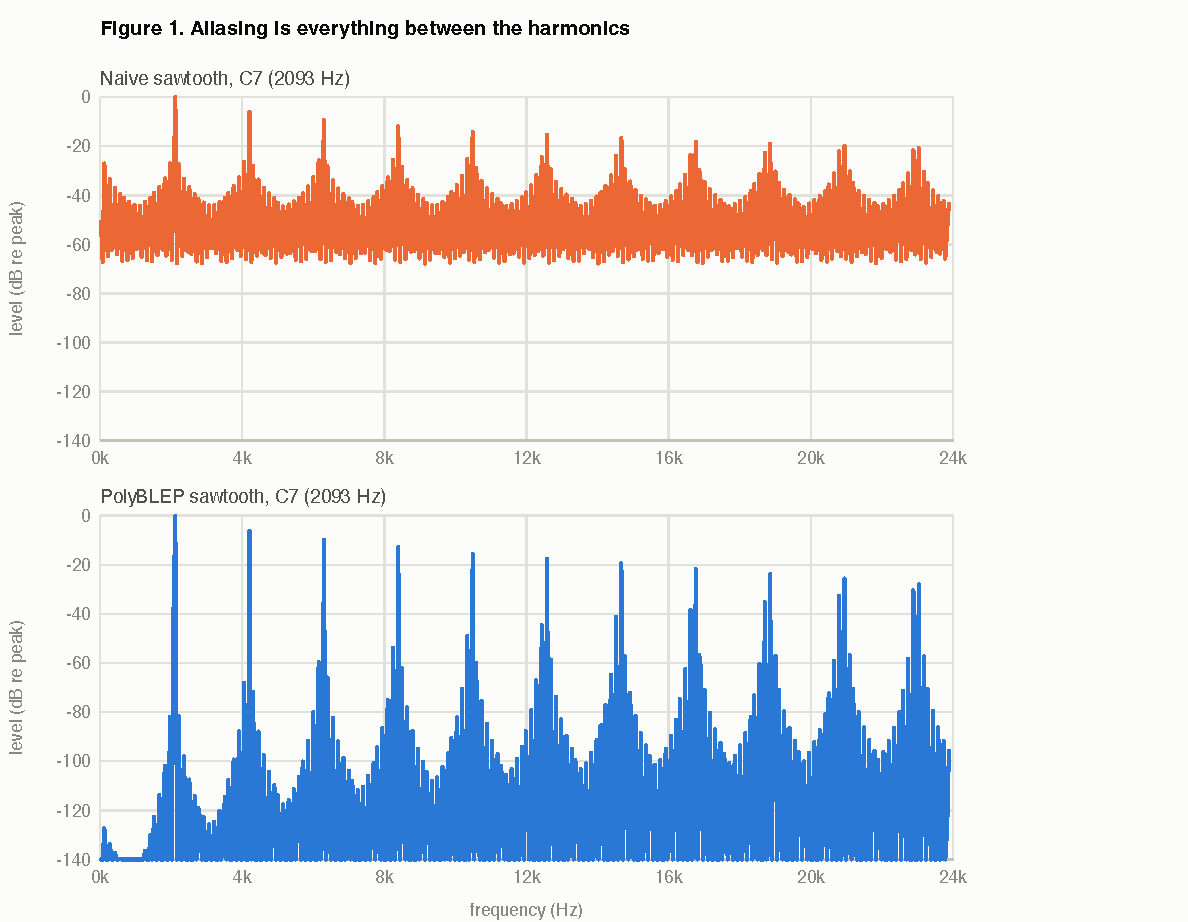
\includegraphics[width=0.84\textwidth]{figures/fig1-spectrum-naive-polyblep.pdf}
\end{figure*}

\begin{figure*}[t]
\centering
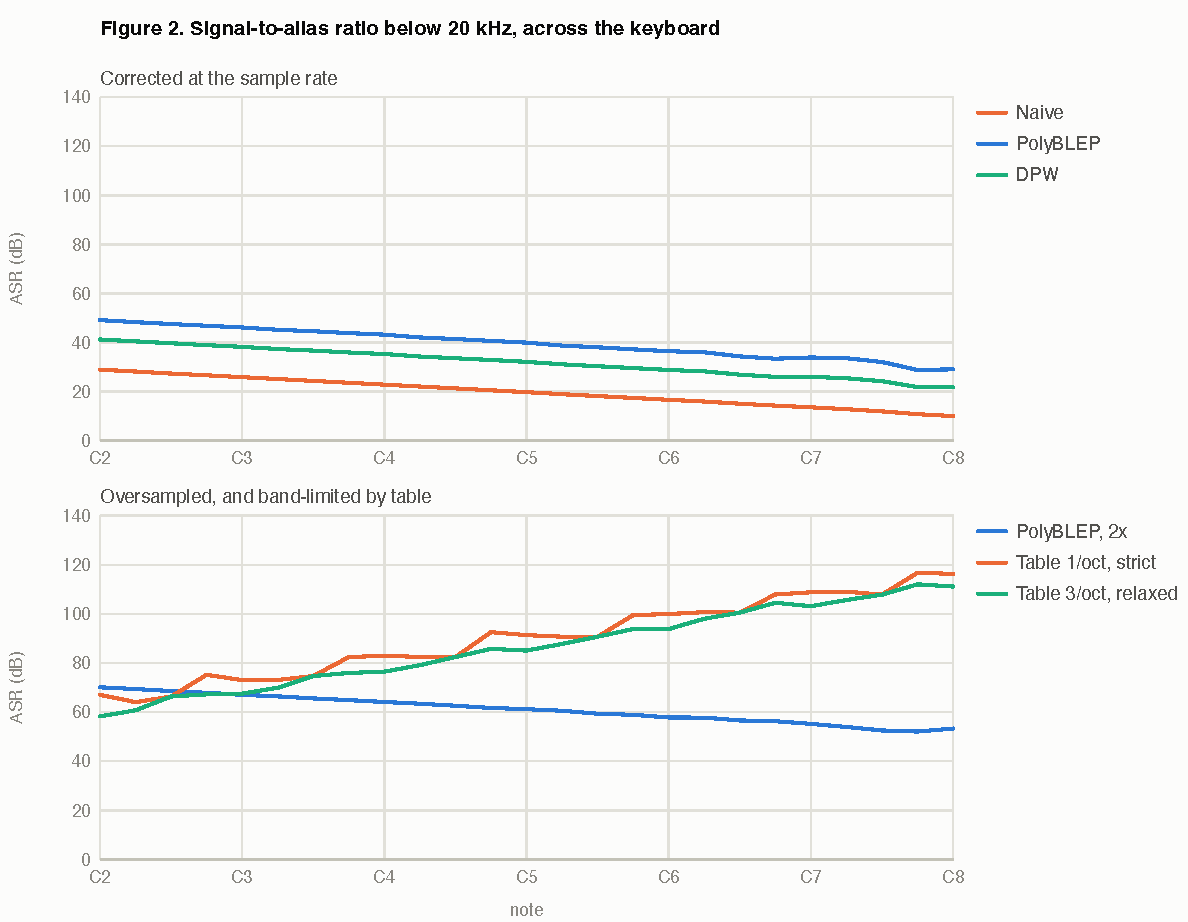
\includegraphics[width=0.84\textwidth]{figures/fig2-asr-keyboard.pdf}
\end{figure*}

\textbf{Naive.} The trivial sawtooth is unusable above the bass register. Its audible ASR falls from 26 dB at C3 to 10 dB at C8, and Figure 1 shows why: at C7 the folded components fill the band to within 20–40 dB of the harmonics.

\textbf{PolyBLEP} gains 15–20 dB everywhere for a cost that, in this harness, is indistinguishable from the trivial saw's (section 4.6).

\textbf{DPW} gains 10 dB at C3, exactly the improvement reported in its original paper \cite{r36}. It falls 6–8 dB short of PolyBLEP across the range.

\textbf{Correction is not removal.} Both correction methods lose about 3–4 dB per octave of pitch, because more of each harmonic series lies near Nyquist where the polynomial approximations are poorest. This is the regime where the literature's higher-order kernels earn their cost: the 4-point B-spline PolyBLEP extends the perceptually alias-free range from about 2.1 kHz to 7.8 kHz \cite{r40}.

\textbf{2× oversampling.} Running PolyBLEP at 96 kHz and decimating with the half-band of section 3.8 buys another 21–24 dB in the audible band. Its whole-band figure is lower because the half-band's transition region, 21.1–26.9 kHz, lets components between 24 kHz and 26.9 kHz fold to between 21.1 kHz and 24 kHz, which is above the audible band.

\textbf{Mip-mapped tables} are in a different class: 68–134 dB across the measured range. Their ASR \emph{rises} with pitch, the opposite of every corrected oscillator. The cause is that the band-limiting is exact, so the residual is whatever the linear interpolation produces. At high pitch the selected level holds few harmonics, each sampled by many table points, and linear interpolation is accurate. At low pitch, the selected level holds hundreds of harmonics, and the top ones have only a few table samples per cycle.

The last row of Table 1 confirms this. The same octave tables at 8192 samples per frame instead of 2048 raise the ASR by 22–25 dB up to C7, the $2 \times 12$ dB that halving the interpolation error twice predicts. The gain shrinks to 18 dB at C8, where the result approaches the measurement's own floor.

\textbf{So for wavetables the lever is the interpolator} (frame size, or a higher-order kernel), not the band-limiting.

\setcounter{subsection}{2}
\subsection{Brightness against aliasing: the wavetable's two parameters}
\begin{table*}[t]
\centering\footnotesize
\caption{Highest harmonic kept by the wavetable, Hz. Strict: ceiling 24 kHz. Relaxed: ceiling 28 kHz, so nothing folds below 20 kHz.}
\begin{tabular}{@{}rrrrrrr@{}}
\toprule
\textbf{MIDI note} & \textbf{f0 (Hz)} & \textbf{1/oct, strict} & \textbf{1/oct, relaxed} & \textbf{3/oct, strict} & \textbf{3/oct, relaxed} & \textbf{below Nyquist} \\
\midrule
60 & 261.6 & 16744 & 16744 & 20930 & 26424 & 23808 \\
62 & 293.7 & 18795 & 18795 & 23493 & 23493 & 23787 \\
64 & 329.6 & 21096 & 21096 & 21096 & 26370 & 23733 \\
66 & 370.0 & 23680 & 23680 & 23680 & 23680 & 23680 \\
68 & 415.3 & 13290 & 26580 & 20765 & 26580 & 23672 \\
70 & 466.2 & 14917 & 14917 & 23308 & 23308 & 23774 \\
72 & 523.3 & 16744 & 16744 & 20930 & 26163 & 23546 \\
\bottomrule
\end{tabular}
\end{table*}

Table 2 shows what each wavetable design gives up: the frequency of the highest harmonic it keeps, against the highest harmonic that could fit below Nyquist.

\textbf{One level per octave, strict ceiling.} This is the textbook design, and it loses up to an octave of top end. At G♯4 the highest harmonic is at 13.3 kHz where 23.7 kHz would fit, so the note sounds audibly duller than its neighbours. The loss repeats at the start of every octave, which makes brightness jump as a melody crosses the boundaries.

\textbf{One level per octave, relaxed ceiling.} Relaxing the ceiling to 28 kHz helps only where the next level's doubled harmonic count happens to fit under it (G♯4 in Table 2). Elsewhere it changes nothing, because one level holds twice the harmonics of the next.

\textbf{Three levels per octave.} Strict, this keeps the loss below a third of an octave. Relaxed, it is the design to prefer. It keeps every note at least as bright as the strict design, and often brighter than an alias-free oscillator could be (26.4 kHz at C4, folding to 21.6 kHz). Table 1 shows its audible ASR within 3 dB of the strict three-per-octave tables and within 6 dB of the octave tables.

\textbf{Memory.} The price of finer spacing is memory. One frame of 2048 samples costs:

\begin{center}\footnotesize
\begin{tabular}{@{}llll@{}}
\toprule
\textbf{Spacing} & \textbf{Levels} & \textbf{Per frame} & \textbf{Per 256-frame table} \\
\midrule
one level per octave & 11 & 88 KiB & 22 MiB \\
three levels per octave & 31 & 248 KiB & 62 MiB \\
\bottomrule
\end{tabular}
\end{center}

At 8192 samples and one level per octave it is 416 KiB per frame and 104 MiB per table.

\textbf{Vital's approach.} This memory cost is a plausible reason for Vital's apparent strategy (section 2.4). Rendering the band-limited frame from its spectrum while playing removes the memory problem and the octave boundaries, and pays in computation instead.

\setcounter{subsection}{3}
\subsection{Filters}
\begin{figure*}[t]
\centering
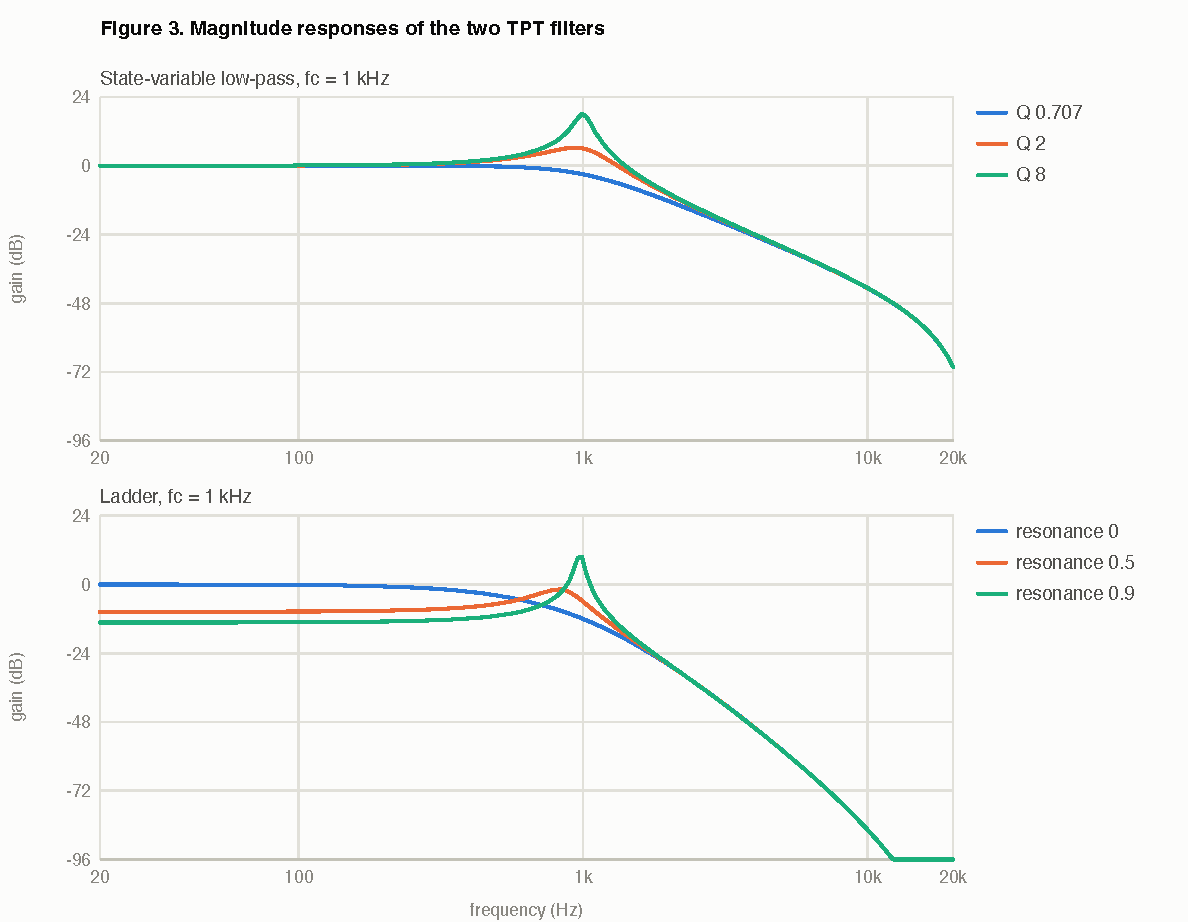
\includegraphics[width=0.84\textwidth]{figures/fig3-filters.pdf}
\end{figure*}

\textbf{Pre-warping.} Figure 3 shows the two TPT filters at 1 kHz. Pre-warping puts the SVF's resonant peak at exactly $20\log_{10} Q$ dB on the cutoff, which is +18 dB at $Q = 8$. Its low-pass slope steepens to a notch at Nyquist, as every bilinear-transformed low-pass does. A filter that must keep its analog slope near Nyquist needs oversampling \cite{r17} or a different discretisation.

\textbf{Ladder passband loss.} The ladder's passband loss is plainly visible: −13 dB at resonance 0.9, i.e. $1/(1+k)$ with $k = 3.6$ \cite{r6,r33}. The cure is a matter of taste:

\begin{itemize}
\item boost the input by $(1+k)$;
\item shape the feedback with a high-pass, so that the bass is not fed back \cite{r42};
\item keep the loss, as the hardware did.
\end{itemize}

\textbf{The cheap nonlinear solution.} The ladder of section 3.6 solves the linear loop and saturates afterwards. It behaves correctly at the edges that matter most: small signals, where it is exact; self-oscillation, where it is bounded; and audio-rate cutoff modulation, where it stays stable. It does not reproduce the way a driven analog ladder's resonance softens as the input level rises, because the \texttt{tanh} never sees the feedback. Getting that right is exactly what the iterative and compensated methods buy \cite{r7,r12,r42}:

\begin{itemize}
\item \textbf{Newton–Raphson:} usually two or three iterations, each needing a \texttt{tanh} and its derivative.
\item \textbf{D'Angelo–Välimäki compensated loop} \cite{r7}.
\item \textbf{D'Angelo–Välimäki circuit model:} 12 more operations per sample than Huovilainen's ladder \cite{r5}.
\end{itemize}

\textbf{Cost.} The modulated ladder costs 39 ns per sample here, the SVF 18 ns (section 4.6).

\setcounter{subsection}{4}
\subsection{Nonlinearities: ADAA and oversampling}
\begin{table*}[t]
\centering\footnotesize
\caption{Waveshaper signal-to-alias ratio, dB, audible band (fs = 48 kHz).}
\begin{tabularx}{\textwidth}{@{}>{\raggedright\arraybackslash}Xrrr@{}}
\toprule
\textbf{Shaper} & \textbf{1047 Hz, drive 4} & \textbf{2093 Hz, drive 4} & \textbf{1047 Hz, drive 16} \\
\midrule
tanh & 91.7 & 51.7 & 33.0 \\
tanh, ADAA & 97.8 & 60.0 & 40.5 \\
tanh, 2x & 139.8 & 124.7 & 72.2 \\
tanh, ADAA + 2x & 139.8 & 134.6 & 86.5 \\
hard clip & 41.8 & 33.5 & 28.7 \\
hard clip, ADAA & 50.6 & 44.2 & 36.4 \\
hard clip, 2x & 56.7 & 48.0 & 43.4 \\
hard clip, ADAA + 2x & 75.3 & 68.2 & 59.2 \\
\bottomrule
\end{tabularx}
\end{table*}

\begin{figure*}[t]
\centering
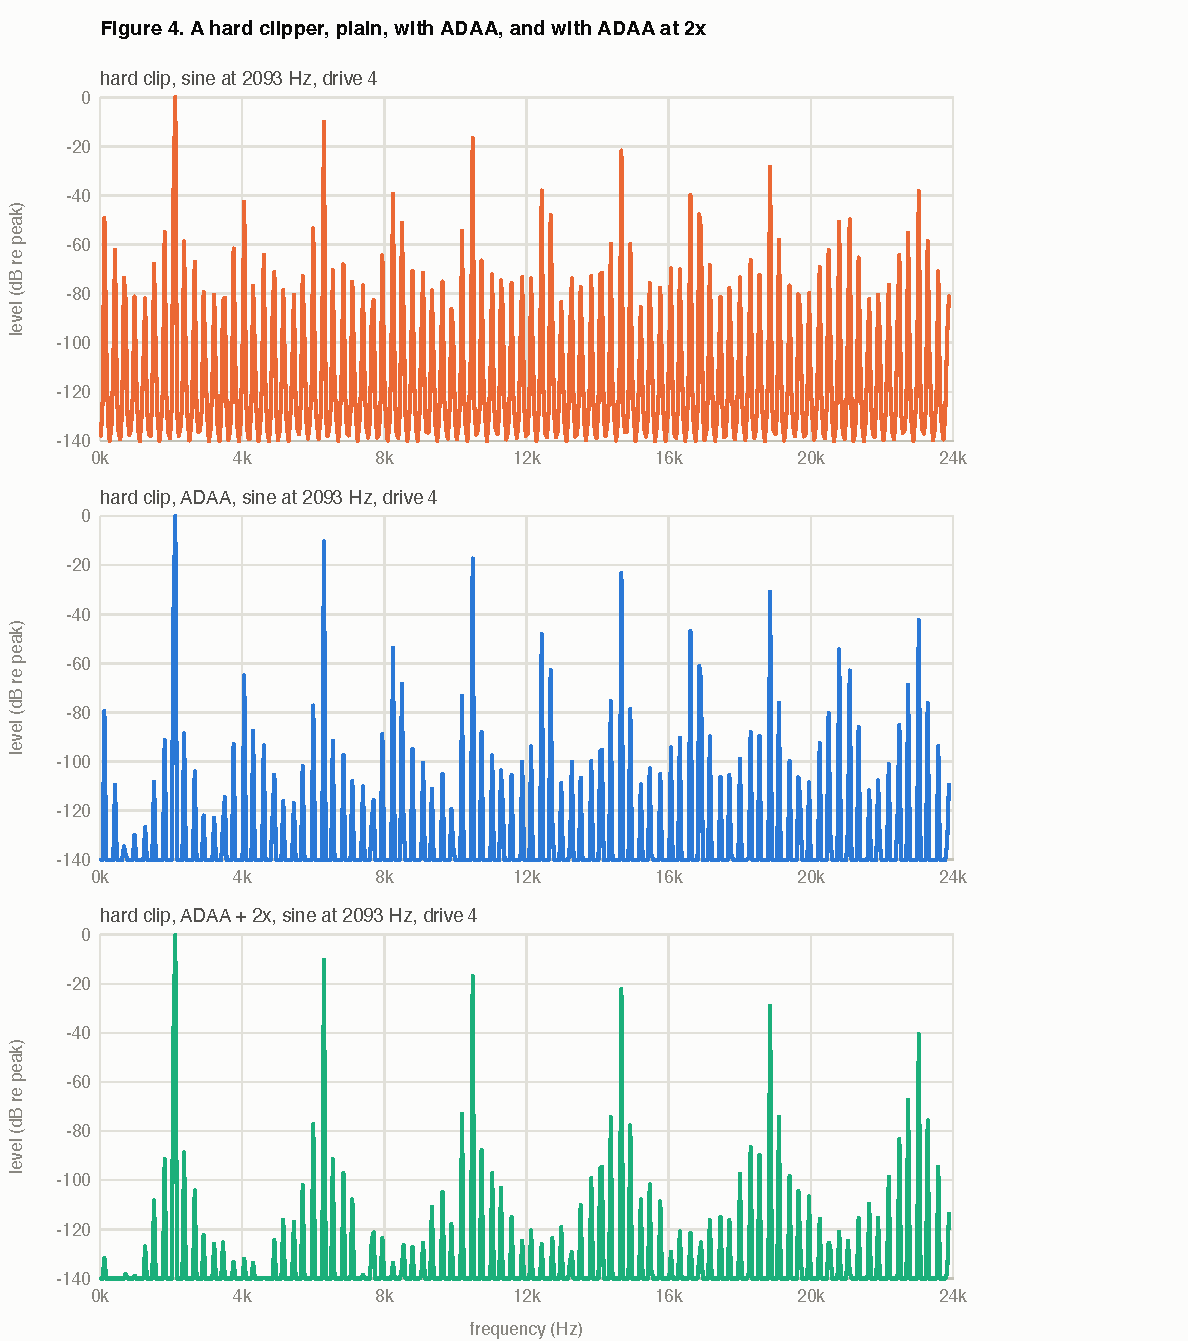
\includegraphics[width=0.68\textwidth]{figures/fig4-shaper-spectra.pdf}
\end{figure*}

Table 3 drives a sine through a \texttt{tanh} and a hard clipper at drives 4 and 16, and Figure 4 shows the hard clipper's spectra at drive 4. Three results stand out.

\textbf{ADAA buys 6–11 dB at 1×.} That is the order of improvement the method promises, and it costs one antiderivative and one division per sample.

\textbf{For a smooth nonlinearity, 2× beats ADAA by a wide margin.} The \texttt{tanh} at drive 4 generates harmonics that fall steeply. Once the rate is doubled, almost nothing reaches the fold-over region, and the ASR jumps from 52 dB to 125–135 dB at 2093 Hz. ADAA at 1× reaches only 60 dB.

\textbf{For a hard clipper, the two combine.} The clipper's corners generate harmonics that fall at only 12 dB per octave. Neither method alone gets past about 57 dB, and ADAA at 2× gains a further 16–20 dB over plain 2×. This mirrors Parker et al.'s result that first-order ADAA lowers the oversampling needed for equal aliasing from 12× to 4× \cite{r25}.

\textbf{Recommendation.} Use 2× oversampling for every waveshaping stage, and add ADAA (higher-order where affordable \cite{r3}) for the shapes with corners: hard clip, folders, rectifiers. This is also why Vital defaults to 2× \cite{S1} and why Serum's ``High'' quality is 2× \cite{S3}.

\setcounter{subsection}{5}
\subsection{Cost}
Median time per sample for each block, from \texttt{cargo bench -p ni-paper-subsynth} (divan, blocks of 4096 samples), on an Apple M1 Pro, single thread, scalar \texttt{f32}, release build:

\begin{table*}[t]
\centering\footnotesize
\begin{tabularx}{\textwidth}{@{}>{\raggedright\arraybackslash}Xr>{\raggedright\arraybackslash}X@{}}
\toprule
\textbf{Block} & \textbf{ns / sample} & \textbf{Notes} \\
\midrule
Trivial saw & 6.4 & the phase accumulator alone \\
PolyBLEP saw & 6.5 &  \\
DPW saw & 6.4 &  \\
Wavetable (2 frames, morph) & 6.4 &  \\
Unison, 7 copies (PolyBLEP) & 12.0 & 1.7 ns per copy \\
TPT SVF, cutoff modulated per sample & 17.6 & includes \texttt{tan} per sample \\
ZDF ladder with \texttt{tanh}, modulated per sample & 39.0 & includes \texttt{tan} and \texttt{tanh} per sample \\
\texttt{tanh} & 6.9 &  \\
\texttt{tanh} with ADAA & 20.7 & \texttt{f64} antiderivative, \texttt{ln}, \texttt{exp} \\
\texttt{tanh} at 2× (half-band up + down) & 50.1 & 2 × 24 MACs each way \\
\bottomrule
\end{tabularx}
\end{table*}

\textbf{The oscillators all cost the same.} This is not a measurement artefact. They are all bound by the same loop-carried dependency, the phase accumulator, and the corrections hide in its latency. Unison shows the other side: seven independent phases overlap and cost 1.7 ns each. \textbf{The lesson for an implementation is to parallelise across voices and unison copies, not within one oscillator.} That is also what Vital's source structure suggests it does, with SIMD vectors that span voices and channels \cite{S1}.

\textbf{Per-sample re-tuning dominates the filters.} A \texttt{tan} per sample costs more than the filter itself. Where the cutoff moves slowly, updating $g$ every 8–32 samples, or reading $\tan$ from a table, is the obvious economy.

\textbf{A voice is far cheaper than a callback.} A PolyBLEP voice with a modulated ladder and an envelope costs about 50 ns per sample. A sample period at 48 kHz is 20.8 µs. Even 32 voices of 7-copy unison stay well inside one core, before any SIMD.

\setcounter{subsection}{6}
\subsection{Problems the oscillator cannot solve on its own}
\textbf{Audio-rate FM and phase modulation.} These spread sidebands without limit and undo any band-limiting done before them. Either limit the index by Carson's rule \cite{r24} or oversample the modulated oscillator.

\textbf{Hard sync.} Every reset of the slave oscillator is a discontinuity at an arbitrary phase. The correction has to be applied there too: BLEP for saw and pulse \cite{r4}, BLAMP for corners \cite{r11}, dedicated residuals for sines \cite{r20}, or spectral methods for wavetables \cite{r27}.

\textbf{Mip-level switching.} A pitch bend that crosses a level boundary changes the harmonic content in one sample, a timbral click. Crossfading between the two levels over a few milliseconds removes it. Finer spacing ($L = 3$) makes each jump smaller.

\textbf{Wavetable warps.} Serum's and Vital's phase-distortion and ``warp'' modes reshape the waveform before it is read. They can reintroduce discontinuities and harmonics above the level's band-limit \cite{S1,S3}. They need the same oversampling as a nonlinearity.

\textbf{Zipper noise.} A parameter applied as a step every block produces a buzz at the block rate. Every parameter that is heard needs a glide (section 3.9).

\textbf{Half-sample delays.} DPW and first-order ADAA each delay the signal by half a sample:

\begin{itemize}
\item harmless in a feed-forward chain;
\item inside a feedback loop the delay detunes the loop, and has to be compensated \cite{r16};
\item mixed against an undelayed path, it causes a comb-filter notch at Nyquist.
\end{itemize}

\setcounter{subsection}{7}
\subsection{Trade-offs at a glance}
\begin{table*}[t]
\centering\footnotesize
\begin{tabularx}{\textwidth}{@{}>{\raggedright\arraybackslash}Xrlll>{\raggedright\arraybackslash}X@{}}
\toprule
\textbf{Method} & \textbf{Audible ASR at C5 (Table 1, 3)} & \textbf{Cost} & \textbf{Latency} & \textbf{Memory} & \textbf{Under modulation} \\
\midrule
Trivial saw & 20 dB & lowest & 0 & 0 & — \\
PolyBLEP & 40 dB & ≈ trivial & 0 & 0 & exact under FM of $f_0$; resets need a residual \\
DPW & 32 dB & ≈ trivial & ½ sample & 0 & start-up transient if not initialised \\
PolyBLEP at 2× & 61 dB & +half-band & 47 samples & 0 & robust \\
Wavetable, 1/oct strict & 91 dB & ≈ trivial & 0 & 88 KiB / frame & dull notes, octave jumps \\
Wavetable, 3/oct relaxed & 85 dB & ≈ trivial & 0 & 248 KiB / frame & bright, small jumps \\
TPT SVF / ZDF ladder & — & 18 / 39 ns & 0 & 0 & time-varying stable \cite{r41} \\
ADAA, order 1 & +6–11 dB & ≈ 3× shaper & ½ sample & 0 & — \\
2× oversampling & +15–73 dB & ≈ 7× shaper & 47 samples & 0 & — \\
\bottomrule
\end{tabularx}
\end{table*}

\setcounter{section}{4}
\section{Summary}
The three discrete-time problems of the subtractive chain each have a mature answer.

\textbf{Discontinuities (P1)} need band-limiting at the source:

\begin{itemize}
\item PolyBLEP for virtual-analog shapes, preferably in its 4-point B-spline form where the extra cost is affordable \cite{r40};
\item mip-mapped tables for wavetables.
\end{itemize}

\textbf{The filter loop (P2)} needs no delay at all. TPT/ZDF filters land on their analog response at the cutoff, stay stable under arbitrary modulation, and cost a few tens of nanoseconds per sample.

\textbf{Nonlinearities (P3)} need oversampling, and ADAA where the nonlinearity has corners.

Measured together, the results recommend the following \textbf{baseline} for a Vital/Serum-class engine, and the crate implements every item except the two upgrades marked \emph{(future)}:

\begin{enumerate}
\item \textbf{Wavetable oscillators:}
\begin{itemize}
\item frames band-limited per level by FFT;
\item three levels per octave, with the relaxed ceiling $f_s - 20$ kHz;
\item frames of at least 2048 samples;
\item linear interpolation \emph{(future: a higher-order interpolator or 8192-sample frames for the bass register)}.
\end{itemize}
\item \textbf{Virtual-analog oscillators:} PolyBLEP, with BLEP residuals at hard-sync resets \emph{(future: the 4-point B-spline kernel)}.
\item \textbf{Unison:} up to 16 copies, $1/\sqrt n$ gain, deterministic spread phases, processed across copies and voices in parallel.
\item \textbf{Filters:} TPT SVF and ZDF ladder, re-tuned per sample where the cutoff is modulated, with the ladder's saturation solved in closed form and Newton iteration as a ``high quality'' option.
\item \textbf{Drive and shapers:} 2× oversampling by half-band FIR as the default quality, as in Vital and Serum, plus first-order ADAA on clipping and folding shapes.
\item \textbf{Voice:} RC-curve envelopes that finish in their stated time and retrigger from their current level, modulation of cutoff in octaves, 5 ms parameter glides, a fixed voice pool with release-first stealing.
\item \textbf{Real time:} nothing allocates while rendering, and a test proves it.
\end{enumerate}

\textbf{Open questions.} Three were left open by this survey:

\begin{itemize}
\item a perceptual rather than spectral comparison of the methods in one harness;
\item how much of the remaining wavetable aliasing a cubic or sinc interpolator removes, per nanosecond spent;
\item whether higher-order ADAA inside a ZDF ladder \cite{r3,r16} can replace oversampling for the filter's own saturation.
\end{itemize}

The code is ready for all three experiments.

\renewcommand{\thesubsection}{\Alph{subsection}}\renewcommand{\thesubsectiondis}{\Alph{subsection}.}
\setcounter{section}{5}
\section{Appendix}
\setcounter{subsection}{0}
\subsection{The DPW scale factor}
The parabola $s^2$, with $s = 2\varphi - 1$, has the Fourier series

\begin{equation*}
s^2(\varphi) = \frac{1}{3} + \frac{4}{\pi^2} \sum_{h=1}^{\infty} \frac{\cos(2\pi h\varphi)}{h^2},
\tag{A1}
\end{equation*}

so its fundamental has amplitude $4/\pi^2$. The first difference $1 - z^{-1}$ has magnitude $2\sin(\omega/2)$ at $\omega = 2\pi f_0/f_s$. For the output's fundamental to equal the ideal saw's, which is $2/\pi$ by Eq. (2), the scale must satisfy

\begin{equation*}
\begin{gathered}
c \cdot \frac{4}{\pi^2} \cdot 2 \sin\!\left(\frac{\pi f_0}{f_s}\right) = \frac{2}{\pi} \\
\Longrightarrow 
c = \frac{\pi}{4 \sin(\pi f_0 / f_s)},
\end{gathered}
\tag{A2}
\end{equation*}

which tends to $f_s/(4 f_0)$ \cite{r36} as $f_0/f_s \to 0$. The test \texttt{it\_\allowbreak{}is\_\allowbreak{}a\_\allowbreak{}unit\_\allowbreak{}saw\_\allowbreak{}at\_\allowbreak{}low\_\allowbreak{}frequency} checks the resulting peak of ±1.

\setcounter{subsection}{1}
\subsection{The trapezoidal integrator and the SVF loop}
The trapezoidal rule integrates $u$ over one sample as

\begin{equation*}
y[n] = y[n-1] + \tfrac{T}{2}\big(u[n] + u[n-1]\big).
\end{equation*}

Pre-warping replaces $\tfrac{T}{2}\omega_c$ by $g = \tan(\pi f_c / f_s)$, so that the digital response equals the analog one at $f_c$. In transposed direct form II, the integrator's output within the sample is $v = g\,u + s$, with state update $s \leftarrow v + g\,u$ (in the listing: \texttt{v1 = g*hp}, \texttt{bp = v1 + s1}, \texttt{s1 = bp + v1}).

\textbf{The SVF loop.} The SVF's high-pass node satisfies $y_{\mathrm{HP}} = x - k\,y_{\mathrm{BP}} - y_{\mathrm{LP}}$. Substituting $y_{\mathrm{BP}} = g\,y_{\mathrm{HP}} + s_1$ and $y_{\mathrm{LP}} = g\,y_{\mathrm{BP}} + s_2 = g^2 y_{\mathrm{HP}} + g\,s_1 + s_2$ gives

\begin{equation*}
y_{\mathrm{HP}}\,(1 + k g + g^2) = x - (k + g)\,s_1 - s_2,
\end{equation*}

which is Eq. (9).

\textbf{The cutoff gain.} At the cutoff the pre-warped digital response equals $H_{\mathrm{LP}}(j) = 1/(jk)$, whose magnitude is $1/k = Q$.

\setcounter{subsection}{2}
\subsection{The ladder's loop solution}
\textbf{The cascade.} A TPT one-pole low-pass computes $v = (x - s)\,G$, $y = v + s$, $s \leftarrow y + v$ with $G = g/(1+g)$. Its output is therefore $y = G\,x + (1 - G)\,s$. Chaining four stages, $y_1 = G u + \sigma_1$, $y_2 = G y_1 + \sigma_2$, and so on, with $\sigma_i = (1-G)\,s_i$, gives

\begin{equation*}
y_4 = G^4 u + \underbrace{G^3\sigma_1 + G^2\sigma_2 + G\sigma_3 + \sigma_4}_{S}.
\end{equation*}

The listing evaluates $S$ by Horner's rule.

\textbf{The loop.} Substituting into $u = x - k\,y_4$ gives Eq. (11).

\textbf{The cutoff gain.} At the cutoff, $s = j$ in Eq. (10) gives $(1 + j)^4 = -4$, so $H(j) = 1/(k - 4)$.

\setcounter{subsection}{3}
\subsection{ADAA as continuous-time convolution}
Let the input be the straight line $\tilde x(t)$ from $x[n-1]$ (at $t = 0$) to $x[n]$ (at $t = 1$). The average of $f(\tilde x(t))$ over the sample is then

\begin{equation*}
\begin{aligned}
\int_0^1 f(\tilde x(t))\,dt &= \frac{1}{x[n] - x[n-1]} \int_{x[n-1]}^{x[n]} f(\xi)\,d\xi \\
&= \frac{F(x[n]) - F(x[n-1])}{x[n] - x[n-1]}.
\end{aligned}
\end{equation*}

This is $f(\tilde x)$ convolved with a one-sample rectangle and sampled at the rectangle's centre. That explains both the low-pass action on what $f$ generates and the half-sample delay \cite{r25}.

\setcounter{subsection}{4}
\subsection{Reproducing the measurements}
From the repository root:

\begin{lstlisting}[language=bash]
cargo test  -p ni-paper-subsynth                          # unit, snippet and no-allocation tests
cargo run   -p ni-paper-subsynth --release --example figures   # figures/*.svg and figures/results.md
cargo bench -p ni-paper-subsynth                          # the cost table of section 4.6
\end{lstlisting}

\textbf{Measurement parameters:}

\begin{itemize}
\item $f_s = 48$ kHz;
\item $2^{17}$ samples analysed, after 4096 samples of start-up;
\item 7-term Blackman–Harris window, harmonic guard of ten bins;
\item audible band 20 kHz;
\item wavetables built from the additive sawtooth of section 3.4.
\end{itemize}

The generated tables are in \texttt{figures/\allowbreak{}results.\allowbreak{}md}. Tables 1–3 of this paper are copied from that file.

\setcounter{subsection}{5}
\subsection{Code map}
\begin{table*}[t]
\centering\footnotesize
\begin{tabularx}{\textwidth}{@{}>{\raggedright\arraybackslash}X>{\raggedright\arraybackslash}X>{\raggedright\arraybackslash}X@{}}
\toprule
\textbf{Listing} & \textbf{Source} & \textbf{Tested by} \\
\midrule
Trivial saw & \texttt{code/\allowbreak{}src/\allowbreak{}osc/\allowbreak{}naive.\allowbreak{}rs\#\allowbreak{}naive} & \texttt{osc::\allowbreak{}naive::\allowbreak{}tests} \\
PolyBLEP saw, pulse & \texttt{code/\allowbreak{}src/\allowbreak{}osc/\allowbreak{}polyblep.\allowbreak{}rs\#\allowbreak{}polyblep}, \texttt{\#\allowbreak{}pulse} & \texttt{osc::\allowbreak{}polyblep::\allowbreak{}tests} \\
DPW & \texttt{code/\allowbreak{}src/\allowbreak{}osc/\allowbreak{}dpw.\allowbreak{}rs\#\allowbreak{}dpw} & \texttt{osc::\allowbreak{}dpw::\allowbreak{}tests} \\
Wavetable frame, levels, reading & \texttt{code/\allowbreak{}src/\allowbreak{}osc/\allowbreak{}wavetable.\allowbreak{}rs\#\allowbreak{}saw\_\allowbreak{}frame}, \texttt{\#\allowbreak{}mip}, \texttt{\#\allowbreak{}read} & \texttt{osc::\allowbreak{}wavetable::\allowbreak{}tests} \\
TPT SVF & \texttt{code/\allowbreak{}src/\allowbreak{}filter/\allowbreak{}svf.\allowbreak{}rs\#\allowbreak{}svf} & \texttt{filter::\allowbreak{}svf::\allowbreak{}tests} \\
ZDF ladder & \texttt{code/\allowbreak{}src/\allowbreak{}filter/\allowbreak{}ladder.\allowbreak{}rs\#\allowbreak{}ladder} & \texttt{filter::\allowbreak{}ladder::\allowbreak{}tests} \\
ADAA & \texttt{code/\allowbreak{}src/\allowbreak{}shaper.\allowbreak{}rs\#\allowbreak{}adaa} & \texttt{shaper::\allowbreak{}tests} \\
Half-band, up, down & \texttt{code/\allowbreak{}src/\allowbreak{}oversample.\allowbreak{}rs\#\allowbreak{}halfband}, \texttt{\#\allowbreak{}up}, \texttt{\#\allowbreak{}down} & \texttt{oversample::\allowbreak{}tests} \\
ADSR & \texttt{code/\allowbreak{}src/\allowbreak{}voice/\allowbreak{}adsr.\allowbreak{}rs\#\allowbreak{}adsr} & \texttt{voice::\allowbreak{}adsr::\allowbreak{}tests} \\
Unison & \texttt{code/\allowbreak{}src/\allowbreak{}voice/\allowbreak{}unison.\allowbreak{}rs\#\allowbreak{}unison} & \texttt{voice::\allowbreak{}unison::\allowbreak{}tests} \\
Allocation & \texttt{code/\allowbreak{}src/\allowbreak{}voice/\allowbreak{}alloc.\allowbreak{}rs\#\allowbreak{}alloc} & \texttt{voice::\allowbreak{}alloc::\allowbreak{}tests} \\
Voice & \texttt{code/\allowbreak{}src/\allowbreak{}voice/\allowbreak{}mod.\allowbreak{}rs\#\allowbreak{}voice} & \texttt{voice::\allowbreak{}tests} \\
All of the above, rendering & — & \texttt{tests/\allowbreak{}no\_\allowbreak{}alloc.\allowbreak{}rs} \\
This document's listings & — & \texttt{tests/\allowbreak{}snippets.\allowbreak{}rs} \\
\bottomrule
\end{tabularx}
\end{table*}

\texttt{tests/\allowbreak{}snippets.\allowbreak{}rs} parses this file. Every \texttt{rust} code block must begin with a comment naming its source as \texttt{/\allowbreak{}/\allowbreak{} <file>\#\allowbreak{}<anchor>}, and the rest of the block must equal the region between \texttt{/\allowbreak{}/\allowbreak{} ANCHOR: <anchor>} and \texttt{/\allowbreak{}/\allowbreak{} ANCHOR\_\allowbreak{}END: <anchor>} in that file. The test also fails if the crate has an anchor this paper never prints.

\setcounter{subsection}{6}
\subsection{Licence and sources}
\textbf{Licences.} The code is © 2026 Torben Gräber and licensed GPL-3.0-or-later. \textbf{Dependencies.} Each dependency's licence is on the repository's allowlist:

\begin{table*}[t]
\centering\footnotesize
\begin{tabularx}{\textwidth}{@{}>{\raggedright\arraybackslash}Xl>{\raggedright\arraybackslash}X@{}}
\toprule
\textbf{Dependency} & \textbf{Licence} & \textbf{Used for} \\
\midrule
\texttt{realfft} & MIT & FFTs \\
\texttt{rustfft} and its own dependencies & MIT OR Apache-2.0 & \texttt{realfft}'s engine \\
\texttt{ni-dsp} & GPL-3.0-or-later & this repository's shared DSP helpers \\
\texttt{assert\_\allowbreak{}no\_\allowbreak{}alloc} & BSD-1-Clause & tests only \\
\texttt{divan} & MIT OR Apache-2.0 & benchmarks only \\
\bottomrule
\end{tabularx}
\end{table*}

\textbf{Clean-room implementation.} No code was taken from any synthesizer or paper. The algorithms were implemented from the equations of the cited publications. Vital's and Surge XT's source trees were consulted only for their documented structure and named constants, and Serum only through its published manual and product page.

\bigskip\noindent
The annotated version, with how each entry was verified, is references.md.

\begin{thebibliography}{99}
\bibitem{r1} D. Ambrits, B. Bank, ``Improved Polynomial Transition Regions Algorithm for Alias-Suppressed Signal Synthesis,'' \emph{Proc. 10th Sound and Music Computing Conf. (SMC 2013)}, Stockholm, pp. 561–568, 2013. doi:\href{https://doi.org/10.5281/zenodo.850287}{10.5281/zenodo.850287}.
\bibitem{r2} R. Bencina, ``Real-time audio programming 101: time waits for nothing,'' blog post, 5 July 2011. \url{http://www.rossbencina.com/code/real-time-audio-programming-101-time-waits-for-nothing}
\bibitem{r3} S. Bilbao, F. Esqueda, J. D. Parker, V. Välimäki, ``Antiderivative Antialiasing for Memoryless Nonlinearities,'' \emph{IEEE Signal Processing Letters}, vol. 24, no. 7, pp. 1049–1053, 2017. doi:\href{https://doi.org/10.1109/LSP.2017.2675541}{10.1109/LSP.2017.2675541}.
\bibitem{r4} E. Brandt, ``Hard Sync Without Aliasing,'' \emph{Proc. Int. Computer Music Conf. (ICMC 2001)}, Havana, pp. 365–368, 2001. \url{https://www.cs.cmu.edu/~eli/papers/icmc01-hardsync.pdf}
\bibitem{r5} S. D'Angelo, V. Välimäki, ``An Improved Virtual Analog Model of the Moog Ladder Filter,'' \emph{Proc. IEEE ICASSP 2013}, pp. 729–733, 2013. doi:\href{https://doi.org/10.1109/ICASSP.2013.6637744}{10.1109/ICASSP.2013.6637744}.
\bibitem{r6} S. D'Angelo, V. Välimäki, ``Generalized Moog Ladder Filter: Part I – Linear Analysis and Parameterization,'' \emph{IEEE/ACM Trans. Audio, Speech, Lang. Process.}, vol. 22, no. 12, pp. 1825–1832, 2014. doi:\href{https://doi.org/10.1109/TASLP.2014.2352495}{10.1109/TASLP.2014.2352495}.
\bibitem{r7} S. D'Angelo, V. Välimäki, ``Generalized Moog Ladder Filter: Part II – Explicit Nonlinear Model through a Novel Delay-Free Loop Implementation Method,'' \emph{IEEE/ACM Trans. Audio, Speech, Lang. Process.}, vol. 22, no. 12, pp. 1873–1883, 2014. doi:\href{https://doi.org/10.1109/TASLP.2014.2352556}{10.1109/TASLP.2014.2352556}.
\bibitem{r8} L. de Soras, ``Denormal numbers in floating point signal processing applications,'' technical note, 2002. \url{http://ldesoras.free.fr/doc/articles/denormal-en.pdf}
\bibitem{r9} F. Esqueda, S. Bilbao, V. Välimäki, ``Aliasing Reduction in Clipped Signals,'' \emph{IEEE Trans. Signal Processing}, vol. 64, no. 20, pp. 5255–5267, 2016. doi:\href{https://doi.org/10.1109/TSP.2016.2585091}{10.1109/TSP.2016.2585091}.
\bibitem{r10} F. Esqueda, H. Pöntynen, J. D. Parker, S. Bilbao, ``Virtual Analog Models of the Lockhart and Serge Wavefolders,'' \emph{Applied Sciences}, vol. 7, no. 12, art. 1328, 2017. doi:\href{https://doi.org/10.3390/app7121328}{10.3390/app7121328}.
\bibitem{r11} F. Esqueda, V. Välimäki, S. Bilbao, ``Rounding Corners with BLAMP,'' \emph{Proc. 19th Int. Conf. Digital Audio Effects (DAFx-16)}, Brno, pp. 121–128, 2016. \url{https://dafx.de/paper-archive/2016/dafxpapers/18-DAFx-16_paper_33-PN.pdf}
\bibitem{r12} F. Fontana, M. Civolani, ``Modeling of the EMS VCS3 Voltage-Controlled Filter as a Nonlinear Filter Network,'' \emph{IEEE Trans. Audio, Speech, Lang. Process.}, vol. 18, no. 4, pp. 760–772, 2010. doi:\href{https://doi.org/10.1109/TASL.2010.2046287}{10.1109/TASL.2010.2046287}.
\bibitem{r13} A. Franck, V. Välimäki, ``Higher-Order Integrated Wavetable Synthesis,'' \emph{Proc. 15th Int. Conf. Digital Audio Effects (DAFx-12)}, York, 2012. \url{https://dafx.de/paper-archive/2012/papers/dafx12_submission_69.pdf}
\bibitem{r14} G. Geiger, ``Table Lookup Oscillators Using Generic Integrated Wavetables,'' \emph{Proc. 9th Int. Conf. Digital Audio Effects (DAFx-06)}, Montréal, pp. 169–172, 2006. \url{https://dafx.de/paper-archive/2006/papers/p_169.pdf}
\bibitem{r15} M. Herlihy, ``Wait-free synchronization,'' \emph{ACM Trans. Programming Languages and Systems}, vol. 13, no. 1, pp. 124–149, 1991. doi:\href{https://doi.org/10.1145/114005.102808}{10.1145/114005.102808}.
\bibitem{r16} M. Holters, ``Antiderivative Antialiasing for Stateful Systems,'' \emph{Applied Sciences}, vol. 10, no. 1, art. 20, 2020 (extended version of the DAFx-19 paper). doi:\href{https://doi.org/10.3390/app10010020}{10.3390/app10010020}.
\bibitem{r17} A. Huovilainen, ``Non-Linear Digital Implementation of the Moog Ladder Filter,'' \emph{Proc. 7th Int. Conf. Digital Audio Effects (DAFx-04)}, Naples, pp. 61–64, 2004. \url{https://dafx.de/paper-archive/2004/P_061.PDF}
\bibitem{r18} J. F. Kaiser, R. W. Schafer, ``On the Use of the I0-sinh Window for Spectrum Analysis,'' \emph{IEEE Trans. Acoustics, Speech, Signal Process.}, vol. 28, no. 1, pp. 105–107, 1980. doi:\href{https://doi.org/10.1109/TASSP.1980.1163349}{10.1109/TASSP.1980.1163349}.
\bibitem{r19} J. Kleimola, V. Välimäki, ``Reducing Aliasing from Synthetic Audio Signals Using Polynomial Transition Regions,'' \emph{IEEE Signal Processing Letters}, vol. 19, no. 2, pp. 67–70, 2012. doi:\href{https://doi.org/10.1109/LSP.2011.2177819}{10.1109/LSP.2011.2177819}.
\bibitem{r20} P. P. La Pastina, S. D'Angelo, ``A General Antialiasing Method for Sine Hard Sync,'' \emph{Proc. 25th Int. Conf. Digital Audio Effects (DAFx20in22)}, Vienna, pp. 109–114, 2022. \url{https://dafx.de/paper-archive/2022/papers/DAFx20in22_paper_3.pdf}
\bibitem{r21} J. Laroche, ``On the Stability of Time-Varying Recursive Filters,'' \emph{J. Audio Eng. Soc.}, vol. 55, no. 6, pp. 460–471, 2007.
\bibitem{r22} H.-M. Lehtonen, J. Pekonen, V. Välimäki, ``Audibility of aliasing distortion in sawtooth signals and its implications for oscillator algorithm design,'' \emph{J. Acoust. Soc. Am.}, vol. 132, no. 4, pp. 2721–2733, 2012. doi:\href{https://doi.org/10.1121/1.4748964}{10.1121/1.4748964}.
\bibitem{r23} J. Nam, V. Välimäki, J. S. Abel, J. O. Smith, ``Efficient Antialiasing Oscillator Algorithms Using Low-Order Fractional Delay Filters,'' \emph{IEEE Trans. Audio, Speech, Lang. Process.}, vol. 18, no. 4, pp. 773–785, 2010. doi:\href{https://doi.org/10.1109/TASL.2009.2035039}{10.1109/TASL.2009.2035039}.
\bibitem{r24} K. Nielsen, ``Practical Linear and Exponential Frequency Modulation for Digital Music Synthesis,'' \emph{Proc. 23rd Int. Conf. Digital Audio Effects (DAFx2020)}, Vienna, pp. 132–139, 2020. \url{https://www.dafx.de/paper-archive/2020/proceedings/papers/DAFx2020_paper_61.pdf}
\bibitem{r25} J. D. Parker, V. Zavalishin, E. Le Bivic, ``Reducing the Aliasing of Nonlinear Waveshaping Using Continuous-Time Convolution,'' \emph{Proc. 19th Int. Conf. Digital Audio Effects (DAFx-16)}, Brno, pp. 137–144, 2016. \url{https://dafx.de/paper-archive/2016/dafxpapers/20-DAFx-16_paper_41-PN.pdf}
\bibitem{r26} P. A. Regalia, S. K. Mitra, P. P. Vaidyanathan, ``The Digital All-Pass Filter: A Versatile Signal Processing Building Block,'' \emph{Proc. IEEE}, vol. 76, no. 1, pp. 19–37, 1988. doi:\href{https://doi.org/10.1109/5.3286}{10.1109/5.3286}.
\bibitem{r27} J. Roth, D. Keller, O. Castañeda, C. Studer, ``Alias-Free Oscillator Synchronization via Additive Synthesis,'' \emph{Proc. 29th Int. Conf. Digital Audio Effects (DAFx26)}, pp. 396–403, 2026. \url{https://dafx.de/paper-archive/2026/papers/DAFx26_paper_49.pdf}
\bibitem{r28} J. Schimmel, ``Audible Aliasing Distortion in Digital Audio Synthesis,'' \emph{Radioengineering}, vol. 21, no. 1, pp. 56–62, 2012. \url{https://www.radioeng.cz/fulltexts/2012/12_01_0056_0062.pdf}
\bibitem{r29} S. Shan, L. Hantrakul, J. Chen, M. Avent, D. Trevelyan, ``Differentiable Wavetable Synthesis,'' \emph{Proc. IEEE ICASSP 2022}, pp. 4598–4602, 2022. doi:\href{https://doi.org/10.1109/ICASSP43922.2022.9746940}{10.1109/ICASSP43922.2022.9746940}.
\bibitem{r30} A. Simper, ``Linear Trapezoidal Integrated SVF,'' Cytomic technical note, 2013 (rev. 2016). \url{https://cytomic.com/files/dsp/SvfLinearTrapOptimised2.pdf}
\bibitem{r31} J. O. Smith III, ``Digital Audio Resampling Home Page,'' CCRMA, Stanford University, 2020. \url{https://ccrma.stanford.edu/~jos/resample/}
\bibitem{r32} T. Stilson, J. O. Smith, ``Alias-Free Digital Synthesis of Classic Analog Waveforms,'' \emph{Proc. Int. Computer Music Conf. (ICMC 1996)}, Hong Kong, pp. 332–335, 1996. \url{https://ccrma.stanford.edu/~stilti/papers/blit.pdf}
\bibitem{r33} T. Stilson, J. O. Smith, ``Analyzing the Moog VCF with Considerations for Digital Implementation,'' \emph{Proc. Int. Computer Music Conf. (ICMC 1996)}, Hong Kong, pp. 398–401, 1996. \url{https://ccrma.stanford.edu/~stilti/papers/moogvcf.pdf}
\bibitem{r34} A. Szabo, \emph{How to Emulate the Super Saw}, B.Sc. thesis, KTH Royal Institute of Technology, report TRITA-CSC-E 2010:131, 2010. Archived at \url{https://web.archive.org/web/20170201235019/https://www.nada.kth.se/utbildning/grukth/exjobb/rapportlistor/2010/rapporter10/szabo_adam_10131.pdf}
\bibitem{r35} R. A. Valenzuela, A. G. Constantinides, ``Digital Signal Processing Schemes for Efficient Interpolation and Decimation,'' \emph{IEE Proc. G}, vol. 130, no. 6, pp. 225–235, 1983. doi:\href{https://doi.org/10.1049/ip-g-1.1983.0044}{10.1049/ip-g-1.1983.0044}.
\bibitem{r36} V. Välimäki, ``Discrete-Time Synthesis of the Sawtooth Waveform With Reduced Aliasing,'' \emph{IEEE Signal Processing Letters}, vol. 12, no. 3, pp. 214–217, 2005. doi:\href{https://doi.org/10.1109/LSP.2004.842271}{10.1109/LSP.2004.842271}.
\bibitem{r37} V. Välimäki, A. Huovilainen, ``Oscillator and Filter Algorithms for Virtual Analog Synthesis,'' \emph{Computer Music Journal}, vol. 30, no. 2, pp. 19–31, 2006. doi:\href{https://doi.org/10.1162/comj.2006.30.2.19}{10.1162/comj.2006.30.2.19}.
\bibitem{r38} V. Välimäki, A. Huovilainen, ``Antialiasing Oscillators in Subtractive Synthesis,'' \emph{IEEE Signal Processing Magazine}, vol. 24, no. 2, pp. 116–125, 2007. doi:\href{https://doi.org/10.1109/MSP.2007.323276}{10.1109/MSP.2007.323276}.
\bibitem{r39} V. Välimäki, J. Nam, J. O. Smith, J. S. Abel, ``Alias-Suppressed Oscillators Based on Differentiated Polynomial Waveforms,'' \emph{IEEE Trans. Audio, Speech, Lang. Process.}, vol. 18, no. 4, pp. 786–798, 2010. doi:\href{https://doi.org/10.1109/TASL.2009.2026507}{10.1109/TASL.2009.2026507}.
\bibitem{r40} V. Välimäki, J. Pekonen, J. Nam, ``Perceptually informed synthesis of bandlimited classical waveforms using integrated polynomial interpolation,'' \emph{J. Acoust. Soc. Am.}, vol. 131, no. 1, pp. 974–986, 2012. doi:\href{https://doi.org/10.1121/1.3651227}{10.1121/1.3651227}.
\bibitem{r41} A. Wishnick, ``Time-Varying Filters for Musical Applications,'' \emph{Proc. 17th Int. Conf. Digital Audio Effects (DAFx-14)}, Erlangen, 2014. \url{https://dafx.de/paper-archive/2014/dafx14_aaron_wishnick_time_varying_filters_for_.pdf}
\bibitem{r42} V. Zavalishin, \emph{The Art of VA Filter Design}, rev. 2.1.2, 2020. \url{https://archive.org/details/the-art-of-va-filter-design-rev.-2.1.2}
\bibitem[S1]{S1} M. Tytel, \emph{Vital}, source repository, GPL-3.0-or-later. \url{https://github.com/mtytel/vital}
\bibitem[S2]{S2} Vital Audio, product site. \url{https://vital.audio/}
\bibitem[S3]{S3} Xfer Records, \emph{Serum 2 User Guide}, version 2.0.18, manual version 1.0.3, 27 April 2025. \url{https://xferrecords.com/manual/serum-2}
\bibitem[S4]{S4} Xfer Records, \emph{Serum} product page, archived 1 January 2024. \url{https://web.archive.org/web/20240101114006/https://xferrecords.com/products/serum/}
\bibitem[S5]{S5} Surge Synth Team, \emph{Surge XT User Manual}. \url{https://surge-synthesizer.github.io/manual-xt/}
\end{thebibliography}
\end{document}
